\chapter{Desarrollo} \label{chp:desarrollo}

La primera parte de este capítulo describe el \textit{modus operandi} del autor de este Trabajo Fin de Grado para contribuir a la librería de modelado fotovoltaico \textit{pvlib-python}, en el que se detallan las herramientas y el entorno de desarrollo empleados.

En el resto de secciones se tratarán las contribuciones de toda índole realizadas, abiertas o planificadas, agrupadas por la temática y la importancia. En aquellas más complejas, se describirán las bases teóricas y se contará el resultado de la propuesta, si es aceptado o no.

\section{Entorno de desarrollo y herramientas utilizadas} \label{sct:desarrollo:entorno}

Para el desarrollo de este trabajo se emplea el siguiente software para el desarrollo del proyecto consistentemente a lo largo de toda su ejecución:

\begin{itemize}
    \item \textit{Visual Studio Code}: es el editor de código que se emplea para escribir y editar el código fuente del proyecto. Es un editor de código semi-abierto, ligero y rápido que cuenta con una amplia gama de extensiones para facilitar el desarrollo de software. Es una alternativa multipropósito a otros editores de código como \textit{PyCharm} o \textit{Spyder} en el caso de Python. Es multipropósito en cuanto admite el desarrollo de muchísimos lenguajes de programación y ficheros ampliamente utilizados en el desarrollo software.
    
    Es importante denotar que la inmensa utilidad que proporciona \textit{VSCode} es gracias a las extensiones creadas por la comunidad de desarrolladores, que permiten desde la edición de archivos de texto plano hasta la depuración del código, pasando por la integración con servicios de control de versiones y la ejecución de tests de forma visual. He aquí extensiones que se emplean en el desarrollo del proyecto:
          \begin{itemize}
              \item \textit{Python}: es la extensión que se emplea para el desarrollo de código en Python. Proporciona funcionalidades como el autocompletado de código, la visualización de la documentación de las funciones, la ejecución de scripts y la depuración de código.
              \item \textit{Ruff}: permite formatear el código según las directrices de estilo de \textit{flake8}, la utilidad que da estilo uniforme al código de Python. Recordemos que establece limitaciones en cuanto a la longitud de las líneas y a la forma de escribir todo el código.
              \item \textit{GitHub Copilot}: un asistente de generación de código en línea integrado en el editor, que se emplea para sugerir fragmentos de código y documentación en función del contexto. Agiliza el desarrollo.
              \item \textit{Code Spell Checker}: es un corrector ortográfico que se emplea para detectar errores de ortografía en el código y en la documentación.
              \item \textit{Jupyter Notebooks}: es la extensión que se emplea para editar y ejecutar \textit{notebooks} de Jupyter en el editor, un formato que permite visualizar las variables del contexto y facilita el debugging interactivo. Los ejemplos de \textit{pvlib-python} se realizan con un formato similar a las celdas de texto o código de una \textit{notebook}.
              \item Resaltado de sintaxis de varios formatos de archivos, como \textit{reStructuredText}, \textit{Markdown}, \textit{YAML} y \textit{TOML}: para facilitar la edición de la documentación y los archivos de configuración.

          \end{itemize}

    \item \textit{GitHub Desktop}: es la interfaz gráfica que se emplea para colaborar en el desarrollo del proyecto. Permite visualizar los cambios, crear \textit{ramas}, hacer \textit{commits}, \textit{pull requests} y \textit{merges}, entre otros. En resumen, administra nuestra copia del repositorio para que los desarrolladores del proyecto puedan revisar y aceptar las propuestas.
    \item \textit{pip} y \textit{venv}: como gestor de paquetes y entornos aislados de desarrollo de Python nativos. Se emplean para instalar las dependencias del proyecto y usar entornos con las versiones específicas requeridas aislado del resto del sistema.


\end{itemize}

De forma discreta, se ha hecho uso de otras herramientas como:

\begin{itemize}
    \item \textit{Git}: para clonar las ramas del autor de este TFG y correr partes de la integración continua, normalmente la documentación, en las máquinas virtuales de linux provistas por la UPM\footnote{Accesible a través de \url{https://escritorio.upm.es/}.}.
    \item \textit{Miniconda}: una distribución de Python que se emplea para instalar y gestionar las dependencias del proyecto. Facilita la creación de entornos virtuales y la instalación de paquetes de Python. Se utilizó para diagnosticar un error de precisión por la compilación de algunas librerías y que hacía fallar un test.
    \item \textit{LibreOffice Calc}: para generar datos de prueba y comprobar las implementaciones de las ecuaciones de los modelos.
\end{itemize}

El desarrollo de la librería se ha hecho habitualmente en Windows 10, en un portátil HP \textit{15-dw2003ns} así que se ha aprovechado a usar el subsistema de Windows para Linux (\textit{WSL}) para ejecutar tests y construir la documentación en un entorno similar al de integración continua. No obstante, por los recursos limitados del portátil, y por poder cambiar de ramas mientras se construye la documentación, se ha hecho uso de las máquinas virtuales de la UPM para ejecutar los tests y construir la documentación.

\subsection{La documentación}

En esta sección pondremos en valor lo que realmente es lo más importante de un proyecto de programación, en especial de código abierto: la documentación. Es más, se puede argumentar que el valor de todas las aportaciones es documentar lo más rigurosamente posible los modelos y métodos que se implementan, tanto para facilitar su correcto uso como para divulgar su existencia y problemática que resuelven.

Como se comentaba anteriormente, la documentación de la librería \textit{pvlib-python} se encuentra alojada en la plataforma \textit{ReadTheDocs}, que expone los archivos HTML para que las personas usuarias puedan consultarla en línea. La documentación se genera automáticamente a partir de los comentarios escritos en el código fuente, que se escriben en formato \textit{reStructuredText} y se construye con el framework \textit{sphinx}.

Existen archivos específicos para indicar qué funciones o métodos son públicos, hacer páginas de inicio, de referencia, de ejemplos, de instalación, de contribución, etc. Además, se pueden incluir imágenes, tablas, gráficos, enlaces, referencias, entre otros elementos que facilitan la comprensión de los conceptos.

\textit{Sphinx} emplea el estilo de documentación de \textit{pydata-sphinx-theme}, que organiza las secciones de la documentación y da un estilo homogéneo a la web. Además, para la creación de los ejemplos se emplea la extensión \textit{sphinx-gallery}, que ejecuta unos scripts de Python por secciones similares a una \textit{notebook} de Jupyter y captura la salida de texto estándar y los gráficos para mostrarlos en la documentación.

La \textit{docstring} de cada función, que es el comentario que se escribe en la primera línea de la definición de la función y se emplea para autogenerar la documentación, utiliza el estilo de \textit{numpydoc}. Este estilo permite incluir información sobre los parámetros de entrada, los valores de retorno, las excepciones que se pueden lanzar, entre otros. Además, se pueden incluir ejemplos de uso de la función e informar avisos de precaución sobre aspectos más específicos.

A continuación se muestra como ejemplo una función mínima con su plantilla de documentación y de código de una función escrita con este fin:

\begin{lstlisting}[language=Python, caption={Ejemplo de documentación de una función en \textit{pvlib-python}.}, label={lst:doc_function_example}]
def example_model(param1, param2):
    """
    Brief model description.

    Long model description, also found at [1]_.

    .. versionadded:: 0.1.0

    .. warning::
       This docstring is an example.

    Parameters
    ----------
    param1 : numeric
      Description of the parameter.
    param2 : numeric
      Description of the parameter.

    Returns
    -------
    float
        Return type of the function.

    Notes
    -----
    Additional notes about the function, detailed explanations if needed. Even an equation:

    .. math::

       f(x, y) = x + y

    Examples
    --------
    >>> example_model(1, 5)
    6.0

    References
    ----------
    .. [1] Author, A. (2024). Title of the paper. Journal, 1(1), 1-10. :doi:`10.0001/populate`
    """
    return float(param1 + param2)
\end{lstlisting}

Esta función, una vez listada en el archivo correspondiente del índice que nos interese -aquí usamos el submódulo \texttt{pvlib.solarposition} como ejemplo-, creará una página como la que se muestra en la figura \ref{fig:doc_function_example}:

\begin{figure}[H]
    \centering
    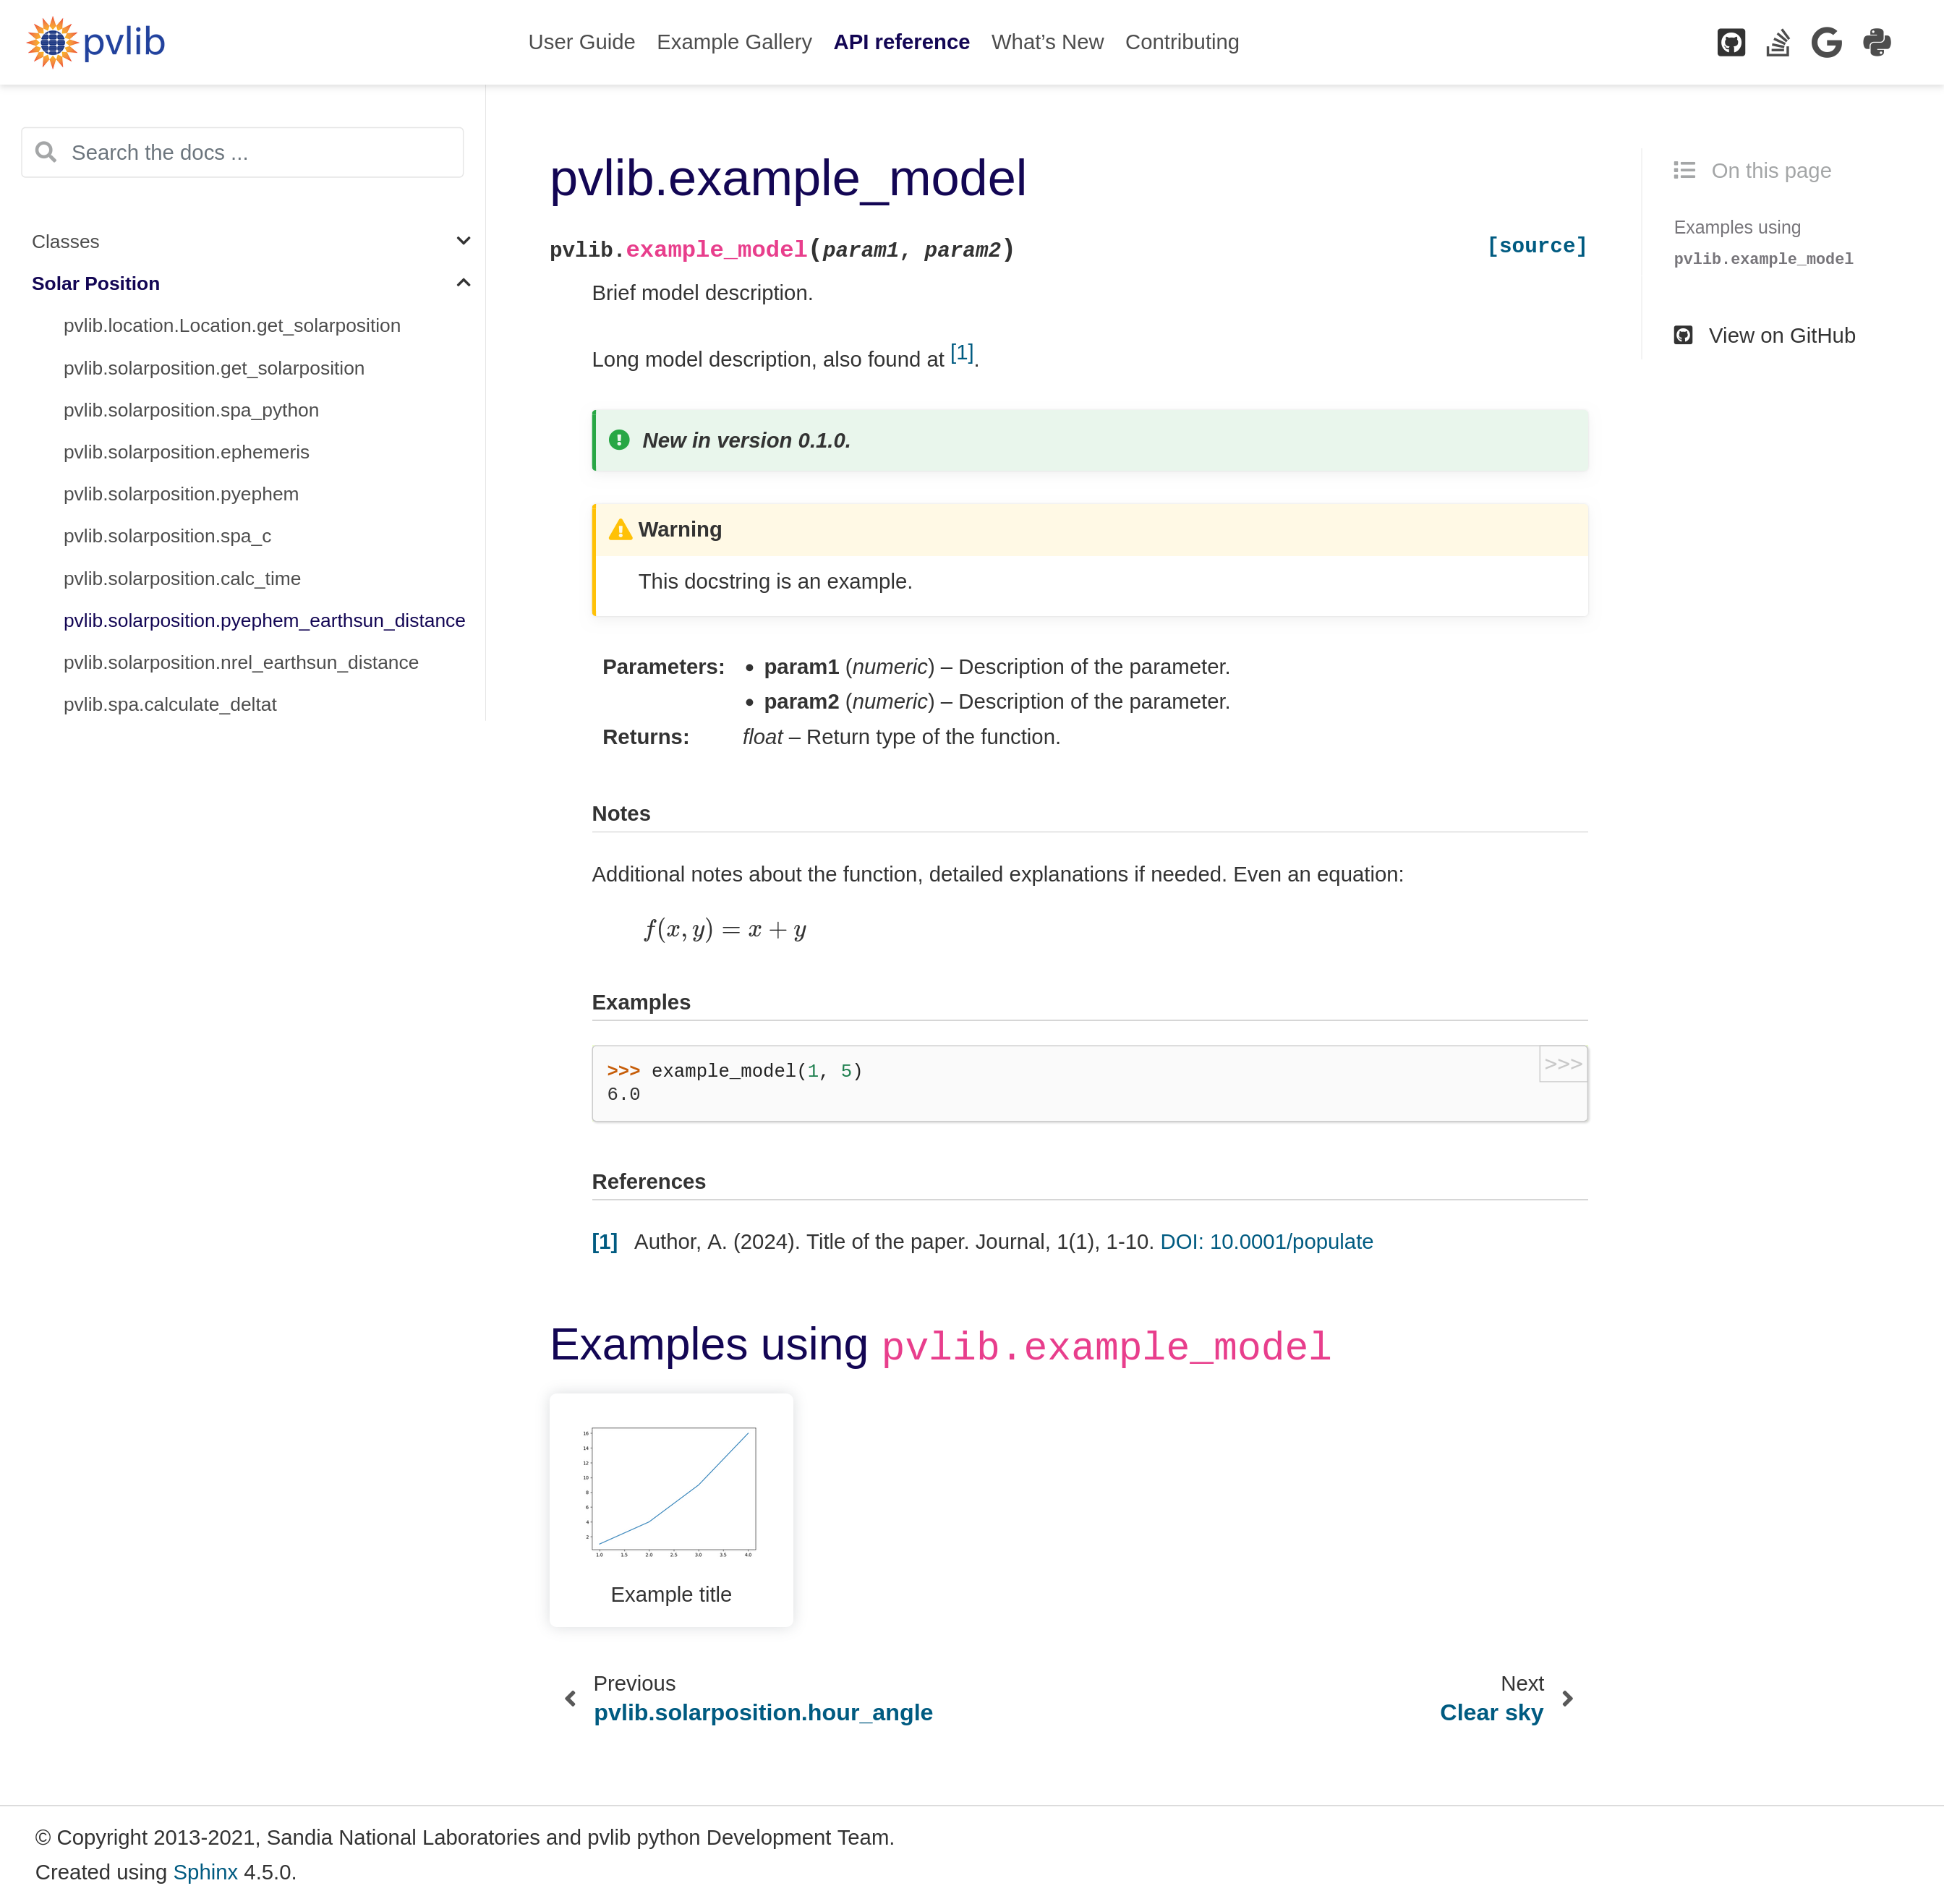
\includegraphics[width=0.9\textwidth]{./images/doc_example/function_stretch.png}
    \caption{Un ejemplo de renderizado de la documentación de una función en \textit{pvlib-python}.}
    \label{fig:doc_function_example}
\end{figure}

Por otro lado, la siguiente estructura pertenece a la redacción de un ejemplo en la documentación. Se emplea para mostrar cómo se usa una función dentro de un contexto más elaborado en cuanto a variables de entrada y salida. Puede incluir todas las características de la documentación de una función:

\begin{lstlisting}[language=Python, caption={Plantilla para elaborar un ejemplo en \textit{pvlib-python}.}, label={lst:doc_example_example}]
"""
Example title
=============

Brief model description (shown in preview card).
"""

# %%
# Text paragraph, in reStructuredText format. Can use sections, subsections, etc., and math as in LaTeX.
# More text.

# This is a comment (there is a newline above)
import matplotlib.pyplot as plt
from pvlib import example_model
print("Hello, world!")
plt.plot([1, 2, 3, 4], [1, 4, 9, 16])
plt.show()

# %%
# Return to paragraph text.

sum_val = example_model(1, 5)
print(f"Sum of 1 and 5 is {sum_val}.")
\end{lstlisting}

El texto anterior constituye un archivo que, ubicado en la carpeta correcta (aquí el archivo es \texttt{docs/examples/solar-position/example\_example.py}), hará que se cree automáticamente una página como la que se muestra en la Figura \ref{fig:doc_use_example}.

\begin{figure}[H]
    \centering
    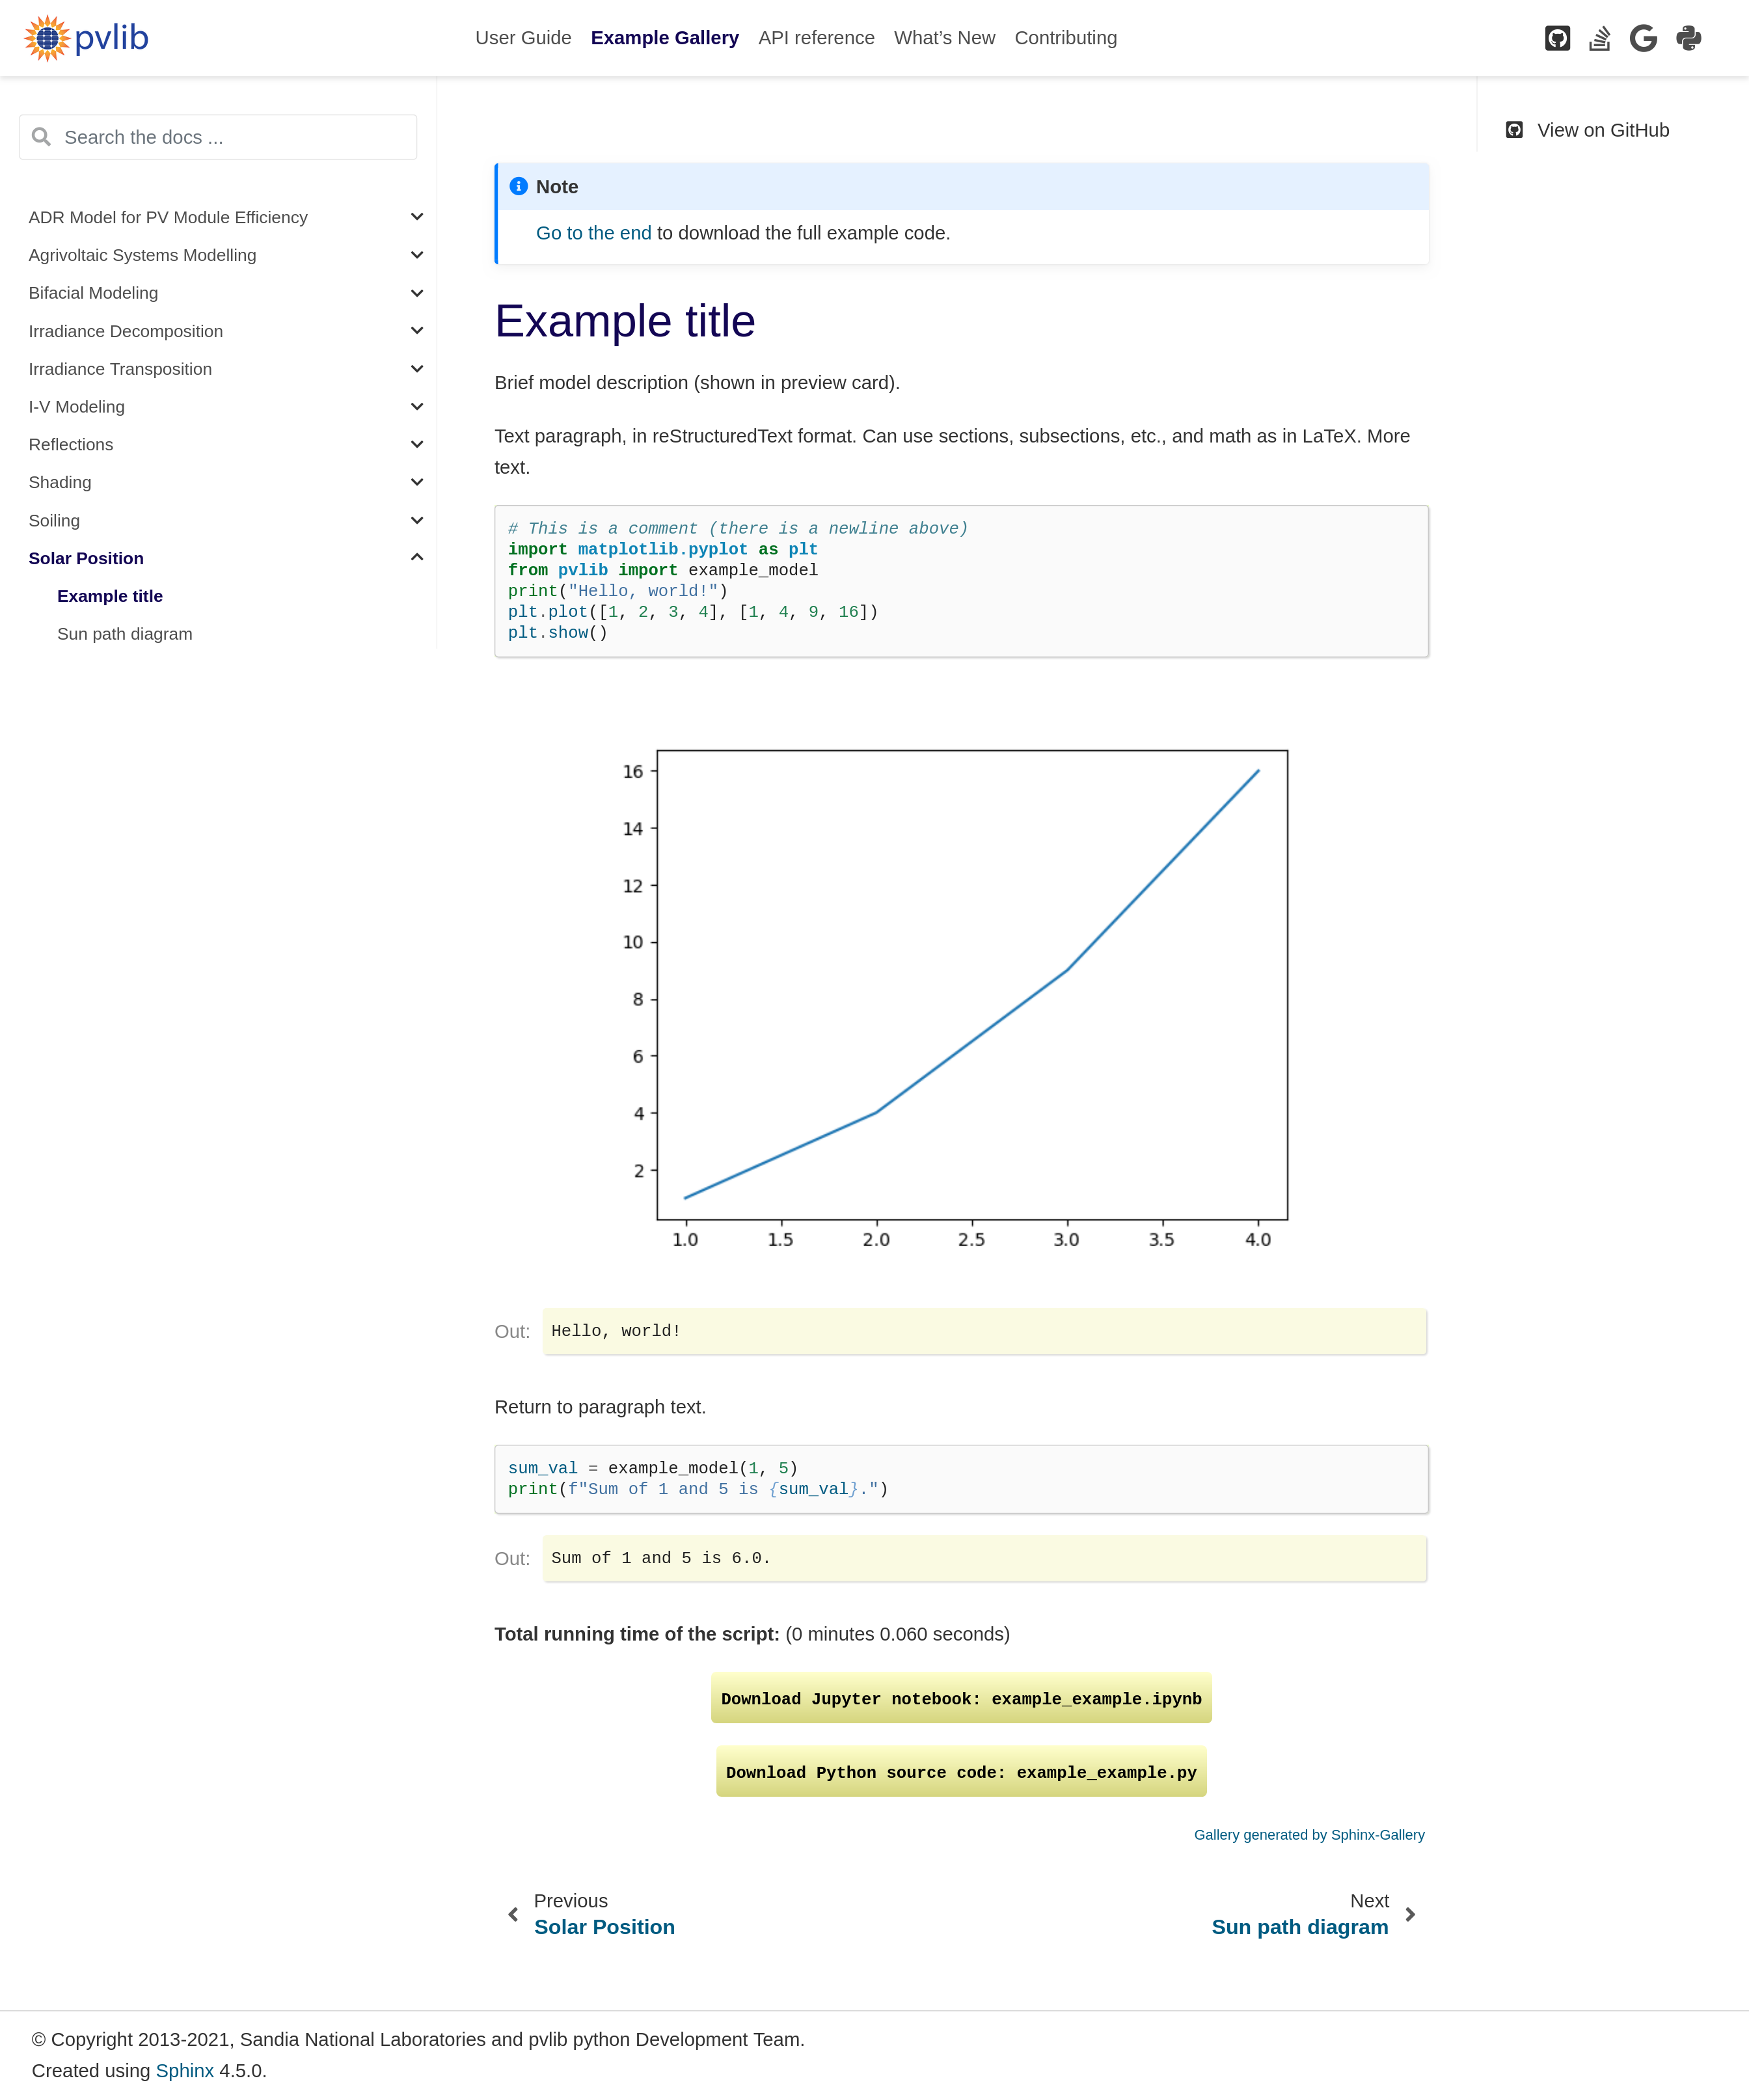
\includegraphics[width=0.9\textwidth]{./images/doc_example/example_stretch.png}
    \caption{Un ejemplo de uso en la documentación de \textit{pvlib-python}.}
    \label{fig:doc_use_example}
\end{figure}

Por último queda construir la documentación. A continuación se muestran los comandos que deben ejecutarse para este fin:

\begin{itemize}
    \item En un sistema basado en \textit{Linux} o \textit{WSL}.
    \item Clonando el repositorio original de la librería con \textit{Git}.
    \item Empleando las mismas versiones que a día de la redacción de este documento se emplea en la integración continua (\textit{pvlib-python=0.11.0}) - en especial hay que hacer la instalación de Python3.8.
    \item Con el entorno aislado de desarrollo (\textit{venv}) activado.
    \item Y realizando una instalación local mediante \textit{pip}.
\end{itemize}

\begin{lstlisting}[language=bash, caption={Comandos para construir la documentación de \textit{pvlib-python}.}, label={lst:doc_build}]
# instalar Python 3.8 desde el repositorio de deadsnakes,
# en las librerias por defecto de Ubuntu no se encuentra disponible por antiguedad
sudo add-apt-repository ppa:deadsnakes/ppa -y
sudo apt-get update
sudo apt-get install python3.8 python3.8-venv -y

# clonar el repositorio de pvlib-python
git clone https://github.com/pvlib/pvlib-python
cd pvlib-python

# crear el entorno virtual, instalar pvlib y las dependencias de la documentacion
python3.8 -m venv .venv
source .venv/bin/activate
python3.8 -m pip install .[doc]

# construir la documentacion
cd docs/sphinx
make html

# abrir la documentacion en el navegador
xdg-open build/html/index.html
\end{lstlisting}

Este conjunto de comandos ha sido ampliamente utilizado para la construcción de la documentación en entornos remotos y así aligerar la utilización de recursos en el portátil personal.

%%%%%%%%%%%%%%%%%%%%%%%%%%%%%%%%%%%%%%%%%%%%%%%%%%%%%%%%%%%%%%%%%%%%%%%%%%%%%%%%%%%%%%
\section{Contribuciones científicas} \label{sct:desarrollo:contribuciones_cientificas}

\subsection{Modelado de ajuste espectral}

\begin{itemize}
    \item \pr{1658}
\end{itemize}

Esta propuesta plantea incluir otro modelo de ajuste espectral, un factor que toma un valor en torno a $1$ y que se emplea para corregir la irradiancia incidente en un módulo fotovoltaico debido a la variación del espectro de la luz solar. El modelo se basa en la tesis doctoral de Nuria Martín Chivelet \cite{Martín_Chivelet_1999} y en un artículo de la misma autora \cite{Martín_Ruiz_1999}.

El desarrollo inició en Septiembre de 2022, en Febrero de 2023 se planteó la \textit{pull request}, que finalmente se cerró en Mayo de 2023 sin incluirse los cambios en la librería al detectar la invalidez del modelo.

\subsubsection{Fundamento teórico}

El modelo \cite{Martín_Ruiz_1999} plantea una relación entre la efectividad bajo un espectro estándar y la efectividad bajo un espectro arbitrario caracterizado por la masa de aire y el índice de claridad. Al principio de la implementación, tanto el autor de este TFG como el mentor del proyecto, César Domínguez, pensaron que se trataba de un modelo de ajuste similar a otros en la literatura que corrigen la irradiancia incidente, para dar lugar a la efectiva. Ejemplos de estos modelos ya se encontraban en la librería, como el modelo desarrollado por la empresa \textit{First Solar} descrito en \cite{Lee_Panchula_2016} o el de Caballero et al. en \cite{Caballero_Fernández_Theristis_Almonacid_Nofuentes_2018}. Además, para la versión 0.11.0 de la librería un compañero del programa \textit{Google Summer of Code} implementó un par de modelos más que funcionan de la misma forma. Los modelos en cuestión crean un factor de ajuste $M$ que se define, según el estándar IEC 60904-7 \cite[Eq. (2)]{Caballero_Fernández_Theristis_Almonacid_Nofuentes_2018}:

\begin{equation}
    M = \frac
    {\int_{\lambda_1}^{\lambda_2} E(\lambda) SR(\lambda) d\lambda \int_{\lambda_3}^{\lambda_4} E^*(\lambda) d\lambda}
    {\int_{\lambda_1}^{\lambda_2} E^*(\lambda) SR(\lambda) d\lambda \int_{\lambda_3}^{\lambda_4} E(\lambda) d\lambda}
\end{equation}

Resultó que, tras un elevado esfuerzo que llevó meses, el modelo en \cite{Martín_Ruiz_1999} no se ajustaba a esta descripción, sino que planteaba la siguiente ecuación:

\begin{equation} \label{eq:ajuste_articulo_Nuria}
    M = \frac{S_{efE(\lambda)}}{S_{ef\bar{G}(\lambda)}}
\end{equation}

Sin embargo, era la fracción de las tres relaciones que se planteaban en la tesis doctoral de Nuria Martín Chivelet \cite{Martín_Chivelet_1999}, que es:

\begin{equation}
    PS = 1 - \frac{S_{efE(\lambda)}}{S_{ef\bar{G}(\lambda)}}\frac{E_{\lambda<\lambda_0}}{\bar{G}_{\lambda<\lambda_0}}\frac{\bar{G}}{E}
\end{equation}

Se puede observar que la ecuación \ref{eq:ajuste_articulo_Nuria} solo contempla una parte de la definición que aplica del ajuste espectral, por ende, invalida la aplicación que se esperaba del modelo de dicho artículo.

Se identifica este error a iniciativa de los tutores pues solicitaron que se comparara este modelo con otros ya implementados en la librería.

\subsubsection{Resultado}

Se descarta aplicar los procedimientos descritos en su tesis \cite{Martín_Chivelet_1999} por:

\begin{itemize}
    \item La ausencia de acceder al documento de forma online.
    \item La ausencia de una versión en inglés, que pueda servir como referencia.
    \item La particularidad de los datos sobre los que se hace el modelo.
\end{itemize}

Lamentablemente, incluso tras contactar presencialmente con la autora y habiendo disfrutado tanto de una explicación detallada de su modelo científico como de la posibilidad de continuar en esa misma línea de trabajo, y contando con una copia física de su tesis, se desestima continuar en esa línea de trabajo debido a las razones anteriores.

Se cierra la propuesta tres meses después de plantearla.

\subsection{Proyección del cenit solar sobre las coordenadas de un colector} \label{sct:desarrollo:contribuciones_cientificas:proyeccion_cenit}

\begin{itemize}
    \item \issue{1734}
    \item \pr{1904}
\end{itemize}

Esta es la primera de una trilogía de contribuciones que se plantean para aplicar un modelo de pérdidas por sombreado en módulos con diodos bypass, cuyo autores pertenecen a la Escuela Técnica Superior de Ingeniería y Diseño Industrial, \textit{ETSIDI}. El objetivo de esta primera contribución es calcular la proyección del cenit solar sobre las coordenadas de un colector, y se utiliza para calcular la fracción de sombra unidimensional en geometrías de paneles que comparten eje de rotación en común.

Las otras dos contribuciones se detallan en \ref{sct:desarrollo:contribuciones_cientificas:fraccion_sombra} y en \ref{sct:desarrollo:contribuciones_cientificas:perdidas_sombreado}.

Esta funcionalidad ya existía como parte de alguna función de la librería, así que el aporte consistió en rehacerla de nuevo empleando una referencia bibliográfica y contrastando las implementaciones. Por supuesto, la documentación conllevó la parte más importante del tiempo de desarrollo.

\subsubsection{Fundamento teórico}

Dos cálculos de bastante interés en geometría solar son obtener los ángulos óptimos de seguimiento  para un colector y calcular la fracción de sombra unidimensional incidente. Ambos cálculos tienen en común un paso muy importante, que es saber con qué ángulo inciden los rayos directos del Sol sobre la superficie del colector, pero referenciado al plano de rotación del mismo.

Para facilitar el entendimiento de este concepto, es preferible imaginar un sistema de rotación de un solo eje. Se puede considerar que un colector fijo, es decir, donde los módulos no rotan, es un caso particular de un seguidor uniaxial. Así será posible definir algunos conceptos más sencillamente.

Nos encontramos estos dos casos de uso:

\begin{itemize}
    \item Para el cálculo de los ángulos óptimos de seguimiento en seguidores de un solo eje, asumiendo que interesa seguir al Sol en su trayectoria diaria, se debe conocer el ángulo de incidencia de los rayos solares sobre la superficie del colector en el plano de rotación del mismo. Es decir, proyectar el cenit solar en el plano perpendicular al eje de rotación del colector, que es aquel que contiene todos los vectores normales al plano del colector.
    \item En el caso de la fracción unidimensional de sombra, interesa saber en donde impactan los límites del colector frontal sobre el trasero. Para ello, se proyecta el cenit solar en el plano perpendicular al eje de rotación del colector, que es aquel que contiene los dos vectores normales a los planos de los colectores.
\end{itemize}

Se puede encontrar en más detalle en el artículo de Lorenzo, Narvarte y Muñoz en \cite{Lorenzo_Narvarte_Muñoz_2011}, personal de la \textit{ETSIDI}, a partir del cual continúa el trabajo de \cite{Anderson_Mikofski_2020}, sección sobre \textit{True-Tracking Angle}. Esta última referencia es ampliamente utilizada a lo largo del repositorio.

\subsubsection{Resultado}

Después de cincuenta y tres comentarios en la propuesta, finalmente se incluyen los cambios como parte de la librería en la versión \texttt{0.10.4}.

Accesible en \linkDocsFunction{pvlib.shading.projected\_solar\_zenith\_angle}.

\subsection{Cálculo de fracción de sombra unidimensional} \label{sct:desarrollo:contribuciones_cientificas:fraccion_sombra}

\begin{itemize}
    \item \issue{1689}
    \item \pr{1962}
\end{itemize}

Esta propuesta es la segunda de la trilogía de propuestas para poder aplicar un modelo de pérdidas por sombreado. Continúa con la propuesta anterior, \ref{sct:desarrollo:contribuciones_cientificas:proyeccion_cenit}, y se encarga de calcular la fracción de sombra unidimensional en paneles con determinadas geometrías.

Aquí se plantea la aplicación de un modelo para conocer la fracción de sombra unidimensional en paneles que comparten eje de rotación en común. La implementación se basa en \cite{Anderson_Jensen_2024}. No obstante, la implementación inició con un póster de una conferencia anterior, a partir de una propuesta de cambios de un trabajador de \textit{First Solar} en la librería \textit{pvlib-python}, que se puede consultar en \url{https://github.com/pvlib/pvlib-python/pull/1725}.

\subsubsection{Fundamento teórico}

El modelo propuesto en \cite{Anderson_Jensen_2024} parte de un diseño de dos colectores de un eje que comparten la misma dirección del eje, y uno se encuentra más cercano al Sol que el otro. Lo interesante de este diseño es que tiene en cuenta múltiples variables de diseño, como la pendiente, la separación entre el eje y el plano colector, e inclinaciones distintas del colector sombreado y el que sombrea.

Se requiere conocer el ángulo proyectado del cenit. A partir de este ángulo, mediante intersección de rectas, se puede conocer la fracción de sombra unidimensional. Realmente se trata de una función muy compleja por el número de entradas que tiene, pues adicionalmente el cálculo de esta proyección se hace internamente en la función para simplificar la API - es decir, la interfaz programática que usarán los usuarios.

Se llama fracción de sombra \textbf{unidimensional} porque mide la fracción de sombra a lo largo de la línea del avance para una misma azimuth pero una elevación solar distinta. Normalmente este valor es el que dota de mayor información, pues los cambios de la sombra debido a la azimuth no cobran tanta importancia en la mayoría de ubicaciones terrestres. Son aquellas latitudes más cercanas a los polos las que más se ven afectados por la cambiante azimuth.

Para facilitar la comprensión de este apartado se muestra un esquema de la sección de dos colectores con distinta inclinación y el ángulo de incidencia solar proyectado, en la imagen \ref{fig:fraccion_sombra}. $f_s$ representa la fracción sombreada del colector 2 por el colector 1:

\begin{figure}[H]
    \centering
    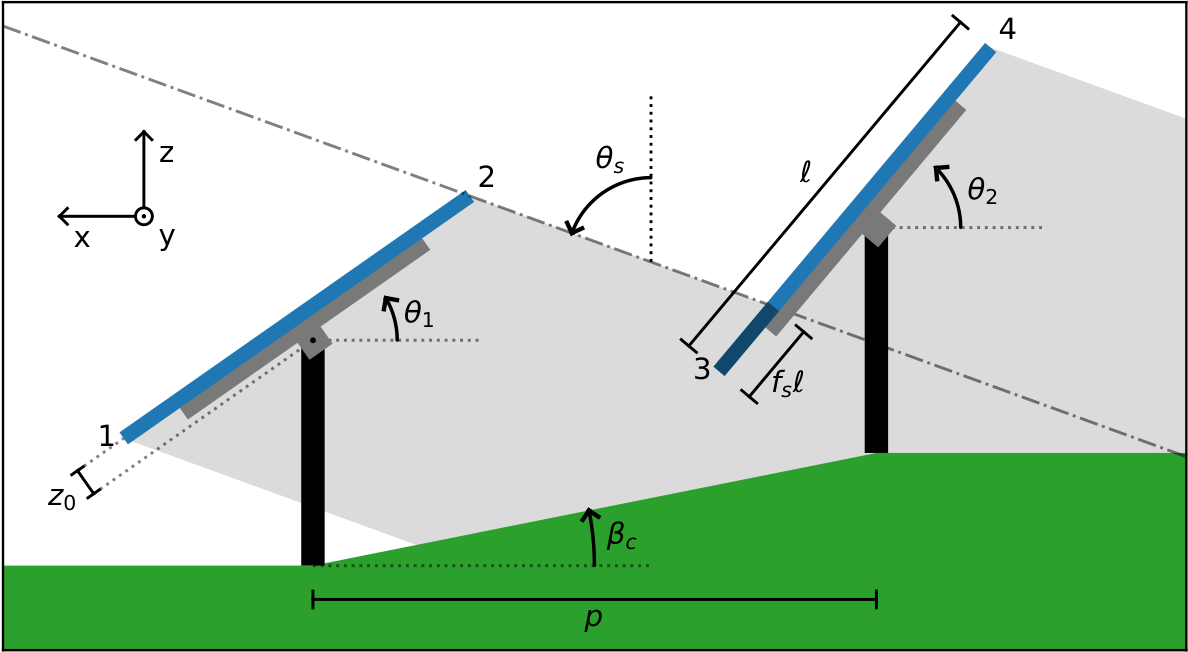
\includegraphics[width=0.6\textwidth]{./images/shading_1d/Anderson_Jensen_Fig3.png}
    \caption{Esquema dos colectores parametrizados, donde uno sombrea al otro. La nomenclatura corresponde la ecuación \ref{eq:sombra_t}.\\Fuente: Figura 3 en \cite{Anderson_Jensen_2024}.}
    \label{fig:fraccion_sombra}
\end{figure}

Las ecuaciones relevantes implementadas son (12) y (13) de \cite{Anderson_Jensen_2024}, \ref{eq:sombra_t} y \ref{eq:sombra_clip} respectivamente en este documento:

\begin{equation} \label{eq:sombra_t}
    \begin{aligned}
        t^* = & \ \frac{1}{2} \left( 1 + \left|\frac{\cos(\theta_1 - \theta_s)}{\cos(\theta_2 - \theta_s)}\right| \right)                                            \\
              & + sgn(\theta_s) \frac{z_0}{\ell} \left( \frac{\sin(\theta_2 - \theta_s) - \sin(\theta_1 - \theta_s)}{\left|\cos(\theta_2 - \theta_s)\right|} \right) \\
              & - \frac{p}{\ell} \left( \frac{\cos(\theta_s - \beta_c)}{\left|\cos(\theta_2 - \theta_s)\right| \cos(\beta_c)} \right)
    \end{aligned}
\end{equation}

\begin{equation} \label{eq:sombra_clip}
    f_s =
    \begin{cases}
        0   & \quad \text{si } t^* < 0 \\
        t^* & \quad \text{si } 0 \leq t^* \leq 1  \\
        1   & \quad \text{si } t^* > 1 \\
    \end{cases}
\end{equation}

\subsubsection{Resultado}

Después de 102 comentarios en la propuesta, finalmente se incluyen los cambios como parte de la librería en la versión \texttt{0.11.0}, junto con un ejemplo ilustrativo que tiene en cuenta posibles dificultades a la hora de utilizarlo\footnote{Véase en \url{https://pvlib-python.readthedocs.io/en/latest/gallery/shading/plot_shaded_fraction1d_ns_hsat_example.html}.}.

Accesible en \linkDocsFunction{pvlib.shading.shaded\_fraction1d}.

Además, como anécdota se ha de mencionar que durante el desarrollo de esta propuesta se identifica la ausencia de ejemplos de módulos orientados al Norte (propio de las instalaciones en el hemisferio Sur) en todo el repositorio, por lo que se añade un ejemplo de este tipo en la documentación.

\subsection{Pérdidas por sombreado en módulos con diodos de bypass} \label{sct:desarrollo:contribuciones_cientificas:perdidas_sombreado}

\begin{itemize}
    \item \issue{2063}
    \item \pr{2070}
\end{itemize}

Con esta propuesta finaliza la trilogía de contribuciones del modelo de pérdidas por sombreado en módulos con diodos de bypass.

La propuesta es de un modelo realizado por personal de la \textit{ETSIDI} y se encarga de calcular las pérdidas por sombreado en módulos con diodos de bypass. La implementación se basa en el trabajo de Martínez-Moreno, F., Muñoz, J. y Lorenzo, E., en \cite{Martínez-Moreno_Muñoz_Lorenzo_2010}.

\subsubsection{Fundamento teórico}

Los módulos de paneles solares de silicio se conforman de múltiples células fotovoltaicas. Una célula, cuando es irradiada por la luz solar, genera una corriente eléctrica. Si conectamos todas las células en serie, la corriente generada por todas las células es la misma, pero la tensión generada por cada célula se suma. Si una célula se sombrea, la corriente generada por ella disminuye, y por tanto la corriente generada por el conjunto también disminuye hasta ser similar a la menor de la producida por cada célula. Esta célula sombreada se comporta como una carga para el resto, pues deben forzar la corriente que pasa por este elemento (que se suele modelar como un diodo). Supone un riesgo de seguridad y de degradación, pues una célula sombreada puede calentarse excesivamente y dañar las capas materiales de su módulo.

La solución que se emplea industrialmente consiste en añadir \textit{diodos de bypass}. Estos permiten que, cuando una serie de células tiene sombra, la corriente mayoritaria generada por el resto de células que están bien iluminadas fluya a través de este diodo, evitando así atravesar la célula sombreada; de esta forma, se protege frente al sobrecalentamiento y la degradación temprana.

Ha de hacerse énfasis en que cada diodo de bypass protege varias células, ya que no es rentable económicamente poner un diodo por cada célula. El planteamiento que nos encontramos en \cite{Martínez-Moreno_Muñoz_Lorenzo_2010} consiste en que, a partir del número de grupos de células protegidos por un diodo que se encuentran sombreados, se puede asumir que el aporte de potencia de este grupo es casi nulo por tener un diodo en conducción y cancelar la potencia proporcional de este grupo frente al total.

\begin{figure}[H]
    \centering
    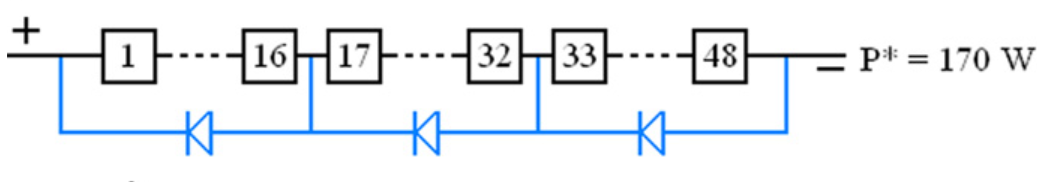
\includegraphics[width=0.6\textwidth]{./images/bypass_diodes/bypass_diodes.png}
    \caption{Esquema de un módulo con 3 diodos de bypass. Si un grupo cuenta con una célula sombreada, el exceso de corriente que no puede fluir a través de ella pasa por el diodo de bypass de su grupo.\\Fuente: Figura 5, a) en \cite{Martínez-Moreno_Muñoz_Lorenzo_2010}.}
    \label{fig:diodos_bypass}
\end{figure}

En la imagen \ref{fig:diodos_bypass}, si suponemos que la célula número 1 está sombreada, la corriente mayoritaria generada por los grupos 17 a 32 y 33 a 48 fluye a través del diodo que está en paralelo con las células 1 a 16. No importa en este caso la corriente del grupo 1 a 16, pues la tensión de este grupo es nula por tener un diodo en conducción.

Nótese que estos grupos se definen en \cite{Martínez-Moreno_Muñoz_Lorenzo_2010} como \textit{bloques}, y según los datos provistos en sus datos originales, un bloque está sombreado en cuanto una de sus células recibe una fracción infinitesimal de sombra.

Lo más complicado de esta contribución es explicar en detalle cómo identificar el número de bloques y su disposición en el módulo, pues existen varias posibilidades. Hay módulos lo suficientemente pequeños para que solo tengan un diodo, los hay con dos y con tres diodos, y los hay \textit{half-cut} que también tienen 3 diodos, pero con una disposición que crea 6 bloques en vez de 3. Además, la progresión de los bloques que se va sombreando depende del sistema y la geometría de las sombras.

El resultado de este modelo establece la cantidad de potencia que se perdería respecto de las mismas condiciones sin sombra, $SL = 1 - \frac{P_\text{sombreado}}{P_{no\,sombreado}}$. Además, anular la potencia de un bloque sombreado se hace sobre la componente directa de la irradiancia, que es la que normalmente genera las sombras, pues la componente difusa sigue impactando en las células sombreadas y creando un mínima parte de aporte energético.

La expresión de pérdidas de potencia es la ecuación \ref{eq:perdidas_sombreado}, Eqs. [6] y [8] en \cite{Martínez-Moreno_Muñoz_Lorenzo_2010}.

\begin{equation} \label{eq:perdidas_sombreado}
    \begin{alignedat}{3}
        (1 - F_{ES}) &= (1 - F_{GS}) \left(1 - \frac{N_{SB}}{N_{TB} + 1}\right) \qquad &\text{(6)}\\
        \left(1 - \frac{P_{S}}{P_{NS}}\right) &= \left(1 - \frac{\left[(B + D^{CIR})(1 - F_{ES}) + D^{ISO} + R\right]}{G}\right) \qquad &\text{(8)}
    \end{alignedat}
\end{equation}

\subsubsection{Resultado}

Tras unos 85 comentarios, finalmente se incluyen los cambios como parte de la librería en la versión \texttt{0.11.0}, junto con un ejemplo de caso de uso\footnote{Véase en \url{https://pvlib-python.readthedocs.io/en/latest/gallery/shading/plot_martinez_shade_loss.html}.}.

Accesible en \linkDocsFunction{pvlib.shading.direct\_martinez}.

\subsection{Fracción diaria de radiación difusa fotosintetizable en función de la fracción difusa global}

\begin{itemize}
    \item \issue{2047}
    \item \pr{2048}
\end{itemize}

Esta contribución se trata de un pequeño modelo que abre un nuevo tema en la librería: la agrivoltaica. La agrivoltaica es una técnica en la que coexisten la producción de energía solar y la producción agrícola en un mismo terreno. La ventaja es que un exceso de irradiancia puede ser perjudicial para la plantación, y el retorno económico del terreno puede ser mayor que si solo se dedicase a la producción de energía solar. Además, disminuye el uso exclusivo de suelo para producción energética, que en ocasiones es un tema controversial.

El modelo en cuestión es la continuación de un trabajo realizado por Spitters C. J. T. et al. que cubre la separación de irradiación en directa y difusa en general \cite{Spitters_Toussaint_Goudriaan_1986}, y que posteriormente él desglosa en dos expresiones en \cite{Spitters_1986}, que se pueden sustituir una en la otra. El objetivo de este modelado es calcular la fracción de irradiación difusa que es útil para las plantas -es decir, fotosintetizable- a partir de la fracción de irradiación difusa global.

\subsubsection{Fundamento teórico}

La irradiación difusa fotosintetizable (\textit{PAR}, por sus siglas en inglés), es la radiación difusa que se encuentra en el rango de longitudes de onda que las plantas pueden absorber y utilizar para la fotosíntesis. Es interesante de cara a simular el crecimiento y producción de las plantas, y se emplea en modelos de cultivo. Esto último queda fuera del alcance de la librería, pero se plantea como un paso para motivar y facilitar el diseño de sistemas agrivoltaicos.

Se utiliza irradiación diaria $[J/m^2/dia]$, en vez del valor instantáneo irradiancia propio de la simulación de sistemas fotovoltaicos $[W/m^2]$.

Un análisis de distintos modelos y la validación de los mismos que contiene la expresión única se puede encontrar en \cite{Ma_Lu_Zainali_Stridh_Avelin_Amaducci_Colauzzi_Campana_2022}, artículo del que origina esta propuesta de contribución inicialmente.

\subsubsection{Resultado}

La mayor complicación de este modelo resultó estar en discernir las unidades de entrada, pues normalmente en fotovoltaica se trabaja con unidades de potencia por unidad de área $\left[W/m^2\right]$, pero aquí se trabaja con energía, $\left[J/m^2\right]$. Finalmente se incluyen los cambios como parte de la librería en la versión \texttt{0.11.0}, junto con un ejemplo de uso\footnote{Véase en \url{https://pvlib-python.readthedocs.io/en/latest/gallery/agrivoltaics/plot_diffuse_PAR_Spitters_relationship.html}.}.

Accesible en \linkDocsFunction{pvlib.irradiance.diffuse\_par\_spitters}.

\subsection{Modelo de pérdidas por heterogeneidad de irradiancia por célula} \label{sct:desarrollo:contribuciones_cientificas:heterogeneidad_irradiancia}

\begin{itemize}
    \item \issue{1541}
    \item \pr{2046}
\end{itemize}

Esta contribución implementa un modelo de pérdidas sobre la potencia de salida para módulos bifaciales, es decir, aquellos que pueden recibir irradiación solar tanto por una cara delantera como por la trasera. El modelo se aplica para tener en cuenta irradiancia que no es homogénea en la superficie del módulo. Se trata del trabajo descrito en \cite{Deline_Ayala_Pelaez_MacAlpine_Olalla_2020}.
Presenta interés en sistemas bifaciales, donde la cara trasera normalmente se expone a la luz reflejada por el suelo y otras obstrucciones, y por tanto la irradiancia de esa cara no es homogénea.

En la cara frontal la irradiancia es mucho más homogénea, así que no se suele tener en cuenta este efecto. No obstante, este modelo se aplica para el valor global de las irradiancias a nivel de célula, o sea, de la suma de la frontal y de la trasera.

\subsubsection{Fundamento teórico}

Anteriormente se explicaba el mecanismo de interconexión de células solares fotovoltaicas, y cómo una célula sombreada puede evitar la producción de energía de las células circundantes. De forma similar ocurre a pequeña escala, cuando una o varias células reciben valores de irradiancia ligeramente distintos al resto. La célula que recibe menos irradiancia limita la corriente, y la potencia de salida del módulo se ve reducida. Sin embargo, por darse en una escala mucho menor, no se puede considerar que la célula sombreada anule la potencia de las demás ya que los diodos de bypass no entran en conducción, sino que simplemente la reduce ligeramente.

Desde un punto de vista computacional, resolver un sistema de múltiples células, cada una con su propia irradiancia, es realmente costoso en tiempo y en recursos. Cada célula tendría su propia curva I-V, que representa cuanta corriente y tensión genera dependiendo del punto de tensión de trabajo. El planteamiento que se hace en \cite{Deline_Ayala_Pelaez_MacAlpine_Olalla_2020} es realizar un trabajo previo de caracterización de la heterogeneidad, cuantificarla y establecer un modelo de menor orden de complejidad.

Para caracterizar distribuciones de irradiancia, en el artículo de Deline et al. \cite{Deline_Ayala_Pelaez_MacAlpine_Olalla_2020} se plantea utilizar la desviación estándar, muy común para distribuciones normales, o la \textit{Diferencia Absoluta Media Relativa} (\textit{RMAD}, por sus siglas en inglés), que es una medida de dispersión que se argumenta ser más adecuada para distribuciones no normales \cite{Ginis_mean_difference_2003}.

La pérdida de potencia de salida $M$ se calcula con un polinomio evaluado en \textit{RMAD}:

\begin{equation} \label{eq:perdidas_heterogeneidad}
    M = 1 - \frac{P_\text{array}}{\sum P_\text{cells}}
\end{equation}

donde $P_\text{array}$ es la potencia de salida del módulo, y $P_\text{cells}$ es la potencia máxima de salida de cada célula.

Se proponen dos modelos para el polinomio que define $M$, para dos perfiles de irradiancias globales distintos: uno para sistemas sujetos fijos y otro para seguidores de un eje. No obstante, solo se implementa el de sistemas fijos ya que la referencia indica que para valores anuales parece ser más preciso.

\subsubsection{Resultado}

Tras involucrarse 7 personas y generar 86 comentarios en los que se plantean distintas formas de implementar el modelo, aclaraciones sobre las unidades de entrada y salida, y modificaciones al planteamiento original, finalmente se incluyen los cambios como parte de la librería en la versión \texttt{0.11.1} (sin publicar oficialmente a día de la redacción de este documento), junto con un ejemplo de uso\footnote{Véase en \url{https://pvlib-python.readthedocs.io/en/latest/gallery/bifacial/plot_irradiance_nonuniformity_loss.html}.}.

Accesible en \linkDocsFunction{pvlib.bifacial.power\_mismatch\_deline}.

Los autores originales del modelo científico piden contrastar la implementación con la suya, y se valora hacerlo en un futuro próximo antes de la siguiente versión de la librería. Se plantea como tarea futura.

\subsection{Transformación de respuesta espectral a eficiencia cuántica externa y viceversa}

\begin{itemize}
    \item \issue{2040}
    \item \pr{2041}
\end{itemize}

Esta contribución podría calificarse de menor debido a la ausencia de dificultades en su implementación. No obstante, por dotar de una nueva funcionalidad científica a la librería, se incluye en este apartado.

La propuesta consiste en dos funciones, una que convierte la respuesta espectral a la eficiencia cuántica externa y otra que hace la operación inversa. Ambas son medidas de la eficiencia de una célula solar para determinadas longitudes de onda de la luz, la primera como corriente generada en función de la potencia recibida y la segunda como la razón de fotones incidentes que generan una corriente eléctrica.

\subsubsection{Fundamento teórico}

La eficiencia cuántica externa es una medida de la eficiencia de una célula solar, y se define como la razón de fotones incidentes que generan una corriente eléctrica para determinado color de la luz. La respuesta espectral es la corriente generada por una célula solar en función de la longitud de onda de la luz incidente.

La relación entre ambas es la siguiente \cite[pp. 15-16, Eq. \brackettext{7}]{Markvart2012-un}:

\begin{equation}
    SR(\lambda) = \frac{q \cdot \lambda}{h \cdot c} \cdot EQE(\lambda)
\end{equation}

\subsubsection{Resultado}

Además de la relación, se añade la posibilidad de normalizar los valores de salida, es decir, hacer que el máximo retornado sea 1. Se incluyen los cambios sin mayores dificultades en la versión \texttt{0.11.0} de la librería.

Accesibles en:

\begin{itemize}
    \item \linkDocsFunction{pvlib.spectrum.qe\_to\_sr}.
    \item \linkDocsFunction{pvlib.spectrum.sr\_to\_qe}.
\end{itemize}

\subsection{Adición de base de datos de respuesta espectral de algunas tecnologías}

\begin{itemize}
    \item \issue{2037}
    \item \pr{2038}
\end{itemize}

Con esta propuesta se pretendía añadir una serie de respuestas espectrales o de eficiencia cuántica externa de células solares de distintas tecnologías comunes, para facilitar la investigación.

\subsubsection{Fundamento teórico}

Una curva de respuesta espectral indica la capacidad que tiene un semiconductor fotovoltaico en convertir la luz incidente en corriente eléctrica en función de la longitud de onda. La eficiencia cuántica externa similarmente es una medida de la eficiencia de una célula solar para convertir fotones en pares electrón-hueco.

Dependiendo de la tecnología de cada material, la respuesta varía. Además, se puede argumentar que otros aspectos constructivos también afectan, como los espesores de las capas y la presencia de impurezas.

\subsubsection{Resultado}

La propuesta no se llegó a añadir en la librería ya que los datos provistos de un repositorio público (en Duramat\footnote{Véase \url{https://www.osti.gov/biblio/2204677}.}) no estaban respaldados por un procedimiento que garantizase que los datos fueran representativos. Tras unas semanas sin mostrarse interés en la propuesta se solicita retroalimentación para tomar una decisión y procede a cerrarse.

\subsection{Adición de espectro estándar completo ASTM G173-03}

\begin{itemize}
    \item \issue{2039}
    \item \pr{1963}
\end{itemize}

Esta adición plantea añadir las componentes de irradiancia directa y extraterrestre del estándar ASTM G173-03, que es un espectro de referencia para la radiación solar en la superficie terrestre. La componente global ya se encontraba en la librería. Se aprovecha para añadir flexibilidad y prevenir la adición de nuevos estándares, como el similar ASTM G173-23 en un futuro.

\subsubsection{Fundamento teórico}

Un espectro estándar es de gran utilidad para comparar módulos y establecer métodos idénticos para tomar las medidas en la industria. En el caso del espectro estándar ASTM G173-03, se establecen una serie de puntos entre los 280 nm y los 4000 nm que simulan una distribución espectral bastante plausible.

La irradiancia extraterrestre es la irradiancia que se recibe en el espacio, y la irradiancia directa es la irradiancia que se recibe en la superficie terrestre sin ser dispersada por la atmósfera, y la global es toda la que se recibe en la superficie terrestre.

El estándar ASTM G173-03 se encuentra en \cite{astm_g173-03}, pero los valores del espectro están disponibles abiertamente en \url{https://www.nrel.gov/grid/solar-resource/spectra-am1.5.html}.
La nueva revisión ASTM G173-23 se encuentra en \cite{astm_g173-23}, pero no cuenta con datos abiertos en la red a día de la redacción de este documento.

\subsubsection{Resultado}

Esta implementación permite obtener el estándar completo y todas sus componentes, lo que hace que la antigua función que solo devolvía la componente global quede obsoleta (\linkDocsFunction{pvlib.spectrum.get\_am15g}). Se aportan cambios y se añaden tests para asegurar que la función obsoleta se elimina adecuadamente en el futuro.

Se incluyen los cambios en la versión \texttt{0.11.0} de la librería, junto con un ejemplo en la documentación\footnote{Véase en \url{https://pvlib-python.readthedocs.io/en/stable/gallery/spectrum/plot_standard_ASTM_G173-03.html}.}.

El ejemplo se puede encontrar en la figura \ref{fig:espectro_astm_g173-03}.

\begin{figure}[H]
    \centering
    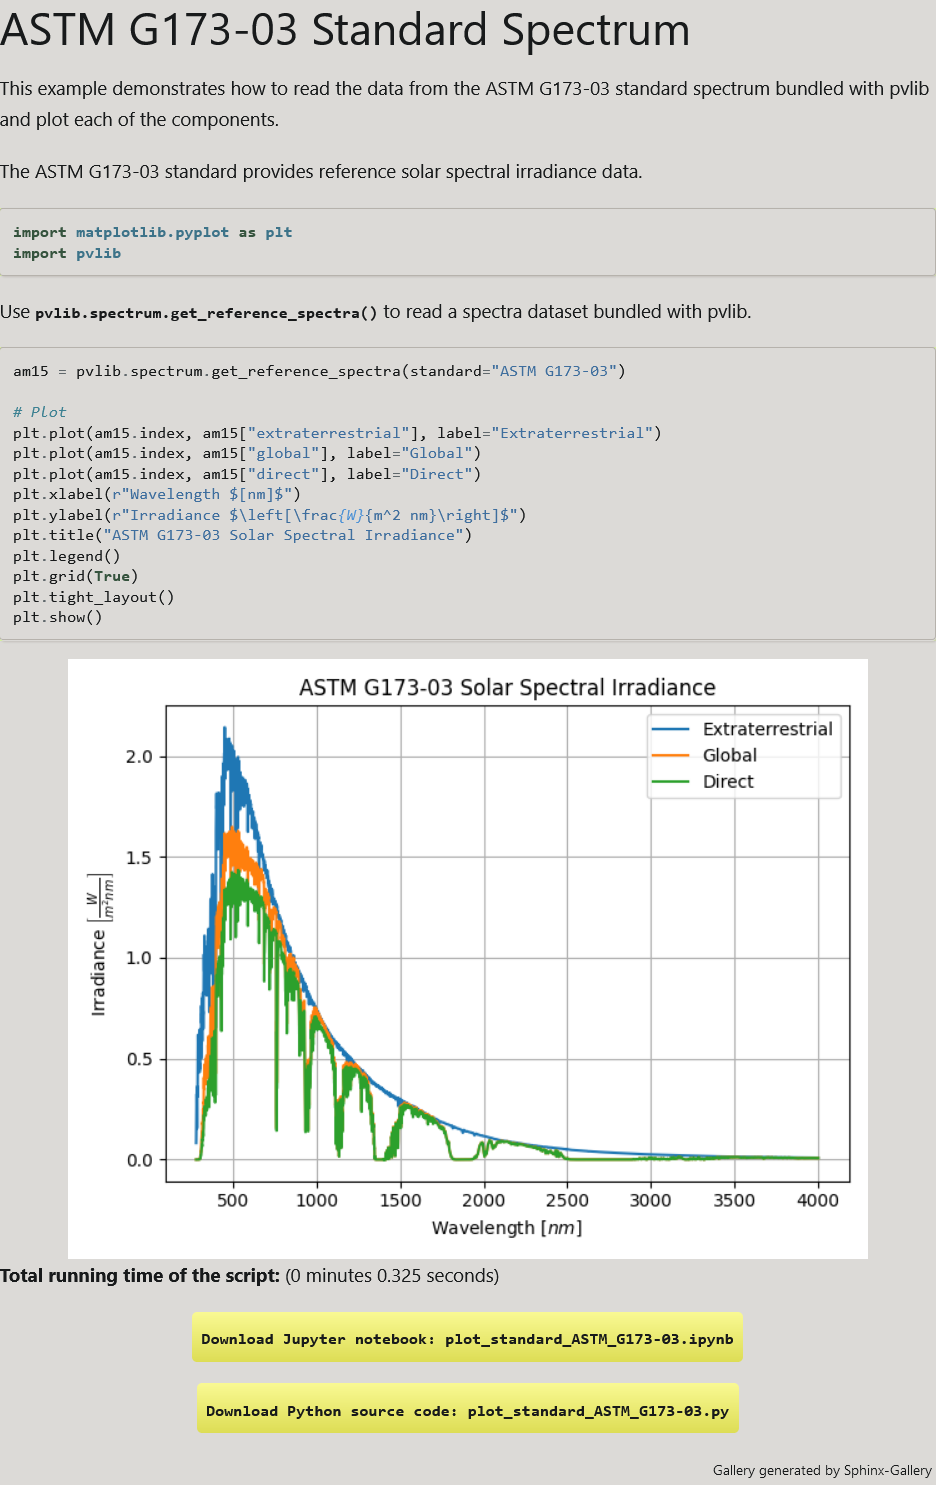
\includegraphics[width=0.8\textwidth]{./images/spectra/astm-g173-03.png}
    \caption{Ejemplo en la documentación con el espectro estándar ASTM G173-03 completo.}
    \label{fig:espectro_astm_g173-03}
\end{figure}

Accesible en \linkDocsFunction{pvlib.spectrum.get\_reference\_spectra}.

\subsection{Cálculo geométrico de sombras en 3D}

\begin{itemize}
    \item \issue{2069}
    \item \pr{2106}
\end{itemize}

Se ha podido comprobar que el cálculo de sombras en sistemas fotovoltaicos dentro de \textit{pvlib-python} es un tema de interés que gracias a este TFG se ha mejorado. Adicionalmente, se ha podido comprobar que la librería no cuenta con una función que permita calcular sombras a partir de objetos en 3D, pero realmente parece ser un tema sobre el que hay literatura. Además, \textit{PVsyst}, un software de simulación de sistemas fotovoltaicos ampliamente conocido cuenta con esta funcionalidad.

Todo esto se puede explorar en un artículo sobre el sombreado de campos de cultivo en sistemas agrivoltaicos \cite{Zainali_Ma_Lu_Stridh_Avelin_Amaducci_Colauzzi_Campana_2023}.

La propuesta que aquí se hace realiza una generalización del cálculo de sombras a superficies limitadas y libres en el espacio 3D.

Es importante denotar que el valor de esta propuesta está pendiente de contar con el interés positivo del grupo, en especial por la extensión del código y la adición de algunas modificaciones al procedimiento del artículo original. Actualmente cuenta con opiniones divididas al respecto.

\subsubsection{Fundamento teórico}

Para esta contribución es imprescindible aplicar conceptos de geometría y cálculo vectorial:

\begin{itemize}
    \item Definición de una recta a partir de un punto y un vector.
    \item Intersección de una recta con un plano.
    \item Traslación de puntos.
    \item Rotación de puntos respecto del origen, mediante matrices de rotación o representación de ángulos de Euler.
    \item Limitar superficies a determinadas coordenadas de otro plano.
\end{itemize}

No se ahonda en estos detalles que generalmente nos brindan algunas librerías de cálculo científico en Python, como \textit{NumPy}, \textit{SciPy} y \textit{Shapely}:

\begin{itemize}
    \item \textit{NumPy} para operaciones con vectores y matrices de forma muy veloz.
    \item \textit{SciPy} para cálculos matemáticos más complejos, particularmente en este caso para hacer rotaciones según que convención se desee, y aplicarla rápidamente mediante el uso de cuaterniones, una manera de representar de rotaciones más compacta y veloz computacionalmente.
    \item \textit{Shapely} para operaciones geoespaciales (según un modelo topológico que permite operaciones geométricas con polígonos). En este caso, se emplea para limitar las sombras a una superficie de interés y representar los objetos de forma uniforme.
\end{itemize}

No obstante, la intersección plano-recta más eficiente y la traslación de puntos no se proporcionan de forma nativa por estas librerías, pero son operaciones que se pueden realizar muy fácilmente con los operadores de Python.

El procedimiento puramente matemático se propone en \cite{Zainali_Ma_Lu_Stridh_Avelin_Amaducci_Colauzzi_Campana_2023}, pero ante todo es necesario priorizar la vectorización del cálculo mediante librerías más rápidas para que sea útil frente al volumen de datos que se suele analizar en simulaciones anuales fotovoltaicas, cuya resolución suele ser horaria como mínimo.

Lo primero que necesita un flujo de trabajo de este tipo es definir coordenadas para los objetos de la escena y sus límites. Para ello, habrá de establecerse un sistema de referencia. En el caso de la propuesta realizada, se opta por cambiar el sistema de coordenadas propuesto en \cite{Zainali_Ma_Lu_Stridh_Avelin_Amaducci_Colauzzi_Campana_2023} por el de \cite{Anderson_Mikofski_2020}, que es más conocido y utilizado en la librería.

Posteriormente, una vez creadas las superficies, tanto las sombreadas como las que generan sombras, se debe calcular el vector de posición solar. Este vector se calcula a partir de la posición del Sol en el cielo, que se puede obtener con la función \linkDocsFunction{pvlib.solarposition.get\_solarposition} y con relaciones trigonométricas.

A continuación, se proyectan los vértices de las superficies que sombrean sobre el plano sombreado, y estos puntos definirán una sombra en la escena 3D. Nótese por tanto que esta sombra puede y debe tener tres coordenadas.

Para obtener la sombra 3D final, debe limitarse los límites de esta a la superficie de interés. Para esto se emplea \textit{Shapely}, que permite realizar operaciones geométricas con polígonos.

Si se desease obtener la sombra en un plano 2D, para realizar otros cálculos y facilitar la visualización, se debe realizar una traslación que ubique la figura en un plano que pase por el origen y unas rotaciones contrarias a las que definen el plano sobre la que se proyectó.

\subsubsection{Resultado}

Ahondando en los detalles, para la resolución de este problema se decide aplicar un paradigma orientado a objectos para facilitar el uso de esta funcionalidad. Se plantean dos objetos:

\begin{itemize}
    \item \texttt{FlatSurface}: una superficie poligonal en el espacio 3D, genérica y que implementa las operaciones que no dependen de la geometría de la superficie, como el cálculo de la sombra que le llega.
    \item \texttt{RectangularSurface}: una especialización de \texttt{FlatSurface} que permite definir superficies rectangulares, que son las más comunes en sistemas fotovoltaicos. En especial, este objeto facilita la creación de superficies a partir de los parámetros más habituales en una instalación fotovoltaica.
\end{itemize}

uno base para cualquier superficie poligonal (\texttt{FlatSurface}) y una especialización para superficies rectangulares, que son las más comunes en sistemas fotovoltaicos (\texttt{RectangularSurface}).

El diagrama UML resultante sería:

\begin{figure}[H]
    \centering
    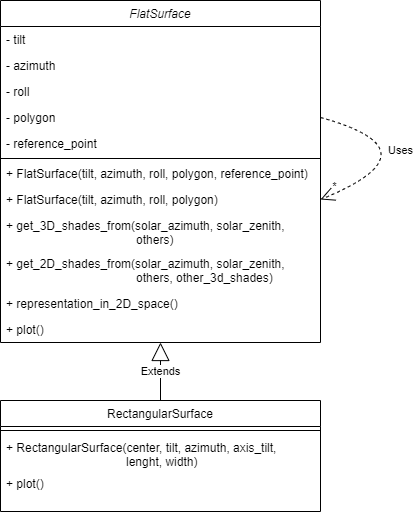
\includegraphics[width=0.8\textwidth]{./images/shading_3d/shading_classes.png}
    \caption{Diagrama UML de la propuesta de cálculo de sombras en 3D.}
    \label{fig:uml_sombreado}
\end{figure}

La elección de un diagrama tan sencillo no es arbitraria: aquí prima la simplicidad y la facilidad de revisar el código para determinar si tiene valor o no dentro de la librería \textit{pvlib-python}. Y realmente se logra sintetizar la API con un buen compromiso entre lo automatizado y la intervención de una persona usuaria. Véase el ejemplo elaborado a continuación:

\begin{lstlisting}[language=Python, caption={Caso de uso de ejemplo para la propuesta de cálculo de sombras en 3D.}, label={lst:sombreado_3d}]
from pvlib.spatial import RectangularSurface
import matplotlib.pyplot as plt
from mpl_toolkits.mplot3d.art3d import Poly3DCollection
import shapely

solar_azimuth = 165  # degrees
solar_zenith = 75  # degrees

# Define two rows of panels
row1 = RectangularSurface(  # south-most row
    center=[0, 0, 3], azimuth=165, tilt=20, axis_tilt=10, width=2, length=20
)

row2 = RectangularSurface(  # north-most row
    center=[0, 3, 3], azimuth=165, tilt=30, axis_tilt=10, width=2, length=20
)

# Calculate shadows
shades_3d = row2.get_3D_shades_from(solar_zenith, solar_azimuth, row1)
shades_2d = row2.get_2D_shades_from(
    solar_zenith, solar_azimuth, shades_3d=shades_3d
)

# Plot
row_style = {"color": "darkblue", "alpha": 0.5}
shade_style = {"color": "dimgrey", "alpha": 0.8}
row_style_2d = {**row_style, "add_points": False}
shade_style_2d = {**shade_style, "add_points": False}

fig = plt.figure(figsize=(10, 10))

# Split the figure in two axes
gs = fig.add_gridspec(10, 1)
ax1 = fig.add_subplot(gs[0:7, 0], projection="3d")
ax2 = fig.add_subplot(gs[8:, 0])

# 3D plot
ax1.view_init(
    elev=60,
    azim=-30,  # matplotlib's azimuth is right-handed to Z+, measured from X+
)
row1.plot(ax=ax1, **row_style)
row2.plot(ax=ax1, **row_style)
for shade in shades_3d.geoms:
    if shade.is_empty:
        continue  # skip empty shades; else an exception will be raised
    # use Matplotlib's Poly3DCollection natively since experimental
    # shapely.plotting.plot_polygon does not support 3D
    vertexes = shade.exterior.coords[:-1]
    ax1.add_collection3d(Poly3DCollection([vertexes], **shade_style))

ax1.axis("equal")
ax1.set_zlim(0)
ax1.set_xlabel("West(-) <X> East(+) [m]")
ax1.set_ylabel("South(-) <Y> North(+) [m]")

# 2D plot
row2_2d = row2.representation_in_2D_space()
shapely.plotting.plot_polygon(row2_2d, ax=ax2, **row_style_2d)
for shade in shades_2d.geoms:
    shapely.plotting.plot_polygon(shade, ax=ax2, **shade_style_2d)

# Calculate the shaded fraction
shaded_fraction = sum(shade.area for shade in shades_2d.geoms) / row2_2d.area
print(f"The shaded fraction is {shaded_fraction:.2f}")
\end{lstlisting}

Debe denotarse que la mayor parte del código supone imprimir la escena y las sombras por pantalla. La parte más interesante, que es el cálculo de las sombras y la fracción sombreada, se reduce a unas pocas 14 líneas de puro código, mientras que se necesitan 27 para mostrar el resultado en 3D y 2D. La escena con las sombras es la que se muestra en la figura \ref{fig:sombreado_3d}:

\begin{figure}[H]
    \centering
    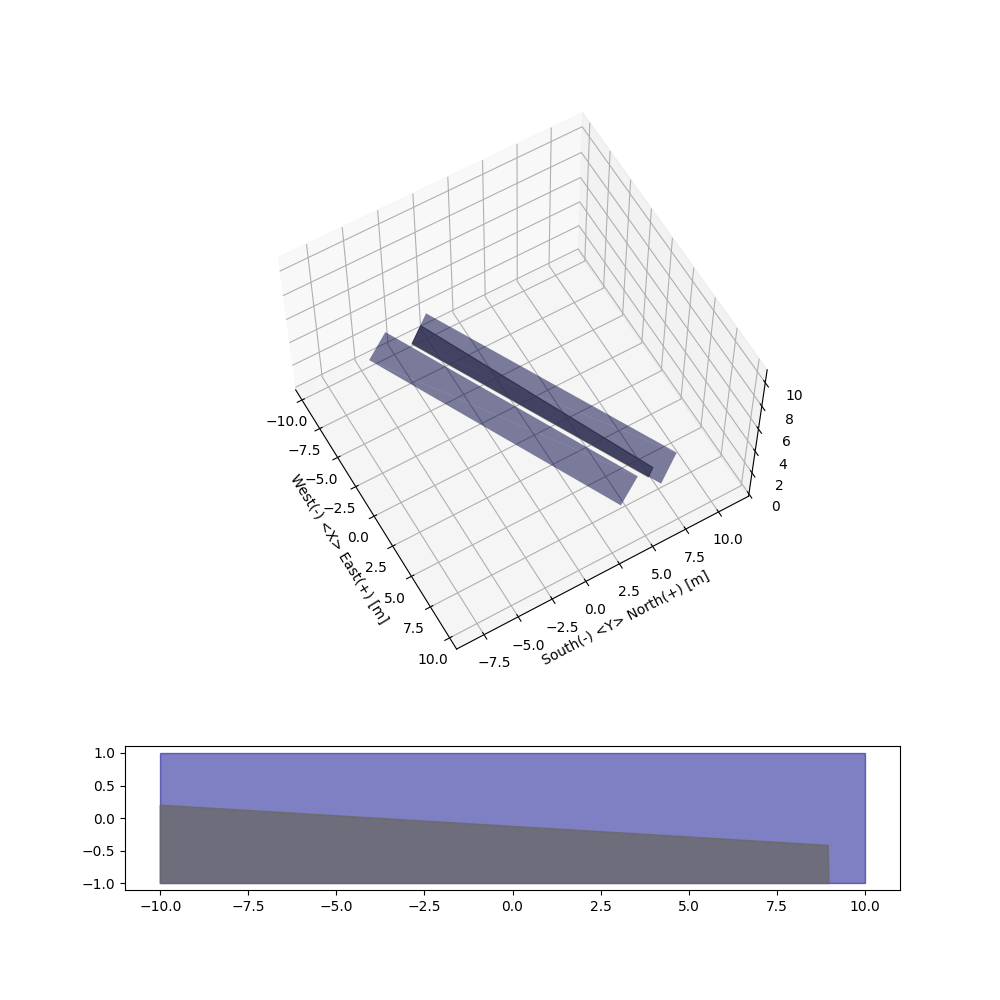
\includegraphics[width=0.8\textwidth]{./images/shading_3d/sphx_glr_plot_spatial_row_to_row_shading_001.png}
    \caption{Ejemplo de sombreado para coordenadas solares instantáneas en 3D.}
    \label{fig:sombreado_3d}
\end{figure}

%%%%%%%%%%%%%%%%%%%%%%%%%%%%%%%%%%%%%%%%%%%%%%%%%%%%%%%%%%%%%%%%%%%%%%%%%%%%%%%%
\section{Contribuciones técnicas} \label{sct:desarrollo:contribuciones_tecnicas}

\subsection{Arreglo a los tests de integración continua en Windows con Conda}

\begin{itemize}
    \item \issue{2000}
    \item \pr{2007}
\end{itemize}

Un test empezó a fallar en la librería, se desconoce las causas, pero solo afectaba a las versiones de la librería cuando se instalaba en Windows con Conda. Este test comprobaba que una curva I-V de una célula solar - esto es, la tensión que aparece en sus terminales en función de la corriente que deja pasar la carga - resultaba válida, y específicamente esperaba que para determinado valor de entrada, la función devolviese un cero prácticamente exacto. Empezó a fallar y retornar un valor igualmente cercano a cero, pero fuera de la tolerancia que se suponía debía de estar.

Algunos de los mantenedores determinaron que no era necesario replantear ni el test ni conocer el motivo la causa, sino que se trataba de un exceso en la precisión que se le pedía al test. Se modificó para que aceptase un margen de error mayor.

Se alega que esto se debió al entorno de pre-compilación de Conda.

\subsubsection{Resultado}

El cambio se incluyó con éxito con bastante rapidez y fue agradecido por los mantenedores del proyecto.

\subsection{Arreglo a un parámetro ignorado en una función de transposición inversa}

\begin{itemize}
    \item \issue{1970}
    \item \pr{1971}
\end{itemize}

Los procedimientos de integración continua supusieron un gran cambio de cara a garantizar la calidad del código en versiones posteriores a la implantación de los mismos. Previo a esto, algunas erratas permanecieron vigentes hasta día de la elaboración de este TFG.

Hoy se identifican fallos de análisis estático en el código nada más hacer una propuesta de cambios. Estos fallos son aquellos que se pueden identificar sin necesidad de ejecutar el código, como el de este caso, que se trataba de un parámetro que no se estaba utilizando en una función.

Este parámetro fue encontrado gracias al resaltado de sintaxis del entorno de desarrollo y se procedió a modificar la función para que cumplir con su propósito: establecer la tolerancia absoluta de convergencia de un método numérico.

El parámetro es \texttt{xtol} de la función \linkDocsFunction{pvlib.irradiance.ghi\_from\_poa\_driesse\_2023}. Esta función hace una transposición inversa, que es deducir la irradiancia global horizontal a partir de la irradiancia en un plano inclinado. El parámetro \texttt{xtol} es la tolerancia absoluta en la convergencia del método numérico y es un factor determinante en el tiempo de ejecución de la función.

\subsubsection{Resultado}

El cambio se incluyó con éxito, aportando tests de integridad para la función y con el agradecimiento del autor original de la función.

\subsection{Dar soporte a otra función para el cálculo del IAM en el flujo orientado a objetos}

\begin{itemize}
    \item \issue{1742}
    \item \pr{1832}
\end{itemize}

El modificador del ángulo de incidencia tiene en cuenta la reflexión de la luz incidente cuando impacta oblicuamente en una superficie transparente. Cuando la radiación es perpendicular a una superficie, se suele considerar que no hay pérdidas ($IAM = 1$), pero conforme el ángulo de incidencia aumenta, debido a la diferencia de índices de refracción una parte de la radiación se refleja, y las pérdidas aumentan ($IAM < 1$).

La librería \textit{pvlib-python} cuenta con muchos modelos que calculan este modificador, pero no todos están disponibles en la \texttt{Modelchain}: un paradigma orientado a objetos que facilita la simulación de sistemas fotovoltaicos.

El modelo al que le faltaba dar soporte era un interpolador de datos ángulo-modificador, \linkDocsFunction{pvlib.iam.interp}. Este toma valores experimentales para, mediante una estimación del valor que se pide, retornar el modificador que cabría esperar. Este interés fue reportado por un usuario donde explicaba que hay estándares para que se provean datos experimentales de este modificador, en vez de los coeficientes que otros modelos necesitan que se aporten.

\subsubsection{Resultado}

El cambio se incluyó con éxito y ahora se encuentra disponible su interfaz en la \texttt{Modelchain}, en \linkDocsFunction{pvlib.modelchain.ModelChain.interp\_aoi\_loss}.

Además, en un plano igual o más importante, se detectó un error en la implementación que ignoraba un parámetro opcional en otro de los modelos que se pueden emplear para simular este efecto.

\subsection{Suprimir una advertencia al publicar la distribución en PyPI}

\begin{itemize}
    \item \pr{1778}
\end{itemize}

Es buena práctica revisar los procedimientos que se realizan automáticamente, ya que con cierta frecuencia dan lugar a advertencias que se ignoran por no ser una cuestión crítica.

Siguiendo este criterio, se revisa manualmente el proceso:

\begin{enumerate}
    \item Ejecución de los tests unitarios: pasan sin nuevos problemas detectados.
    \item Creación de la documentación: no genera advertencias desconocidas anteriormente.
    \item Construcción de la distribución: también pasa sin crear avisos.
    \item Publicación de prueba en TestPyPI: se detecta una advertencia sobre el formato de la descripción que se obtiene de \texttt{README.md}, el archivo de presentación del proyecto.
\end{enumerate}

No se trata de nada crítico: tan sólo es la plataforma PyPI que solicita explícitamente el formato del texto de la descripción del proyecto. Puede aportarse en texto plano, MarkDown o reStructuredText.  % TODO: revisar

\subsubsection{Resultado}

Se suprime adecuadamente la advertencia especificando que el formato es reStructuredText y se añade el cambio propuesto sin mayor discusión.

\subsection{Exponer parámetros de tolerancia para resolver el modelo de un diodo}

\begin{itemize}
    \item \issue{1249}
    \item \pr{1764}
\end{itemize}

Esta contribución da inicio con la solicitud de un usuario que desea modificar los parámetros de tolerancia de unas funciones que resuelven las curvas I-V de las células o módulos fotovoltaicos.

Estas curvas son de especial interés para saber cómo se va a comportar eléctricamente el circuito cuando se conecte una carga, pero la complejidad matemática que suponen hacen que se resuelvan mediante métodos numéricos. Estos métodos son iterativos y requieren de una precisión para converger.

Por defecto esta tolerancia es de $10^{-6}$ [voltios, amperios o vatios], lo que a este usuario le parecía excesivo y quería agilizar el proceso modificando dicho valor. Este caso no es extensible a todos los contextos, pero el planteamiento es completamente válido sobre las hipótesis que plantea el usuario.

\subsubsection{Resultado}

Por un lado, se trabajó directamente en esta propuesta y se planteó. Fue un cambio bienvenido en la librería.

Asimismo, se planteó que de cara a exponer parte del sistema de resolución por métodos numéricos, debía devolverse opcionalmente un objeto del método con información como su convergencia, entre otros.

Este último apartado supuso la mayor dificultad en implementarse, pero se consiguió exitosamente. Se añadieron tests profundos para asegurar que la nueva funcionalidad cumplía con la especificación.

\subsection{Modificar tolerancias erróneas en varios tests unitarios}

\begin{itemize}
    \item \pr{2082}
\end{itemize}

Originalmente la librería empleó un framework de testing que especificaba las tolerancias como número de decimales después de la coma. Al cambiar de framework al nuevo y más moderno \textit{pytest}, no se modificaron estos números para reflejar el nuevo significado de las tolerancias, como un margen absoluto en torno al que deben estar los números.

Supuso que números enteros que representaban número de ceros hasta el primer uno se empezasen a interpretar como una tolerancia absoluta. Por ejemplo, donde antes había un $6$ ahora debía escribirse un $1e-6 = 10^{-6}$.

Existe el riesgo de que estos fallos hubiesen pasado por alto problemas de implementación.

\subsubsection{Resultado}

El cambio se incluyó con éxito, sin diagnosticar ningún fallo derivado de esta errata, garantizando una vez más la integridad y calidad de la librería.

\subsection{Arreglo de un bug que ignoraba parámetros de una función de lectura de bases de datos}

\begin{itemize}
    \item \issue{2018}
    \item \pr{2020}
\end{itemize}

En \textit{pvlib-python} existe la función \linkDocsFunction{pvlib.pvsystem.retrieve\_sam} que permite leer de bases de datos ya inclusas en la librería o remotas mediante una URL, mediante dos parámetros distintos. Resulta que si se especificaban ambos parámetros, solo se leía la base de datos de la distribución, y no la remota, sin emitir ningún aviso.

\subsubsection{Resultado}

Se aplicó un patrón de diseño que excluía la posibilidad de que ambos parámetros se especificasen a la vez, y se incluyó sin dificultades.

\subsection{Actualizar versiones de las dependencias de la documentación}

\begin{itemize}
    \item \pr{2112}
\end{itemize}

Esta contribución se trata de una iniciativa propia dentro de este TFG. Se trata de actualizar las versiones de las dependencias de la documentación, que se construye automáticamente con \textit{Sphinx} y algunas extensiones extras, para dotar de un nuevo \textit{look-and-feel} (o, estilo) a la documentación.

Se prioriza que el renovado entorno pueda pasar el mayor tiempo posible sin generar problemas ni requerir atención.

\subsubsection{Resultado}

Entre las características más destacables de la nueva documentación está el atajo de teclado para realizar búsquedas; tema gráfico para cambiar entre unos colores claros y otros oscuros según la preferencia del lector, y una ubicación un poco más estética de algunos elementos.

Se han aceptado los cambios, que serán visibles en la rama estable de la documentación a partir de la próxima versión \texttt{0.11.1}.

%%%%%%%%%%%%%%%%%%%%%%%%%%%%%%%%%%%%%%%%%%%%%%%%%%%%%%%%%%%%%%%%%%%%%%%%%%%%%%
\section{Contribuciones menores} \label{sct:desarrollo:contribuciones_menores}

Aquí se tratan aquellas que no suponen un desafío ni técnico ni científico, si bien suponen y parten de la interacción en el repositorio y la identificación particular de necesidades.

\subsection{Añadir una utilidad para obtener los ficheros de ejemplo internos de la librería}

\begin{itemize}
    \item \issue{924}
    \item \pr{1763}
\end{itemize}

El objetivo consistió en añadir una función que ahorrase escribir la instrospección de la ubicación de la librería para formar las rutas manualmente.

\begin{lstlisting}[language=python, caption={Fragmento de código utilizado normalmente para obtener la ruta de los ficheros de la librería}, label={lst:example_files_current}]
import os
import pvlib

PVLIB_DIR = pvlib.__path__[0]
DATA_FILE = os.path.join(PVLIB_DIR, 'data', '723170TYA.CSV')
\end{lstlisting}

Concretamente, la propuesta crea una función que se utilizaría como sigue:

\begin{lstlisting}[language=python, caption={Fragmento de código utilizando la función propuesta para obtener la ruta de los ficheros de la librería}, label={lst:example_files_proposal}]
import pvlib

DATA_FILE = pvlib.tools.get_example_dataset_path('723170TYA.CSV')
\end{lstlisting}

Se desestima la propuesta porque se considera que primero deben reorganizarse todos los ficheros de ejemplo, si bien esto último nunca se ha puesto en marcha debido a la inmensidad de la tarea.

\subsection{Corrección de erratas en la documentación}

\begin{itemize}
    \item \pr{1599}
    \item \pr{1860}
    \item \pr{1996}
\end{itemize}

Se han solventado erratas en la documentación, encontradas mayoritariamente de casualidad al navegar entre el código con otros fines.

\subsection{Corrección de erratas en ejemplos y en código}

\begin{itemize}
    \item \pr{1776}
    \item \pr{1833}
\end{itemize}

Son pequeñas modificaciones que no requieren mayor explicación: actualizar la salida desfasada de un ejemplo y comprobar que un único script de ejemplo que no se ejecuta automáticamente fuera capaz de hacerlo localmente.

\subsection{Modificación de escritura de los parámetros opcionales}

\begin{itemize}
    \item \issue{1574}
    \item \pr{1828}
    \item \pr{2084}
\end{itemize}

En Python existe un patrón de diseño que consiste en darle el valor \texttt{None} a los parámetros opcionales, y luego comprobar si efectivamente son \texttt{None} con el fin de asignarles un valor por defecto o ignorarlos si fuese el caso.

Normalmente, a la hora de documentarlo lo recomendable es indicar que el parámetro es opcional, pero lo habitual hasta antes de esta contribución era indicar que el valor por defecto es \texttt{None}, lo cual es redundante y obfusca las intenciones del código.

Se cambiaron todas las ocurrencias de \texttt{default None} a \texttt{optional}, aunque hubo que iterar múltiples veces para dar con todos los falsos negativos y no obtener falsos positivos. Para esta tarea se empleó el buscador en archivos integrado en \textit{Visual Studio Code}, que está basado en \textit{ripgrep} y hace uso de expresiones regulares, una forma de búsqueda y sustitución muy potente: las expresiones regulares son un lenguaje formal que permite buscar patrones en texto, por ejemplo sustituyendo un carácter por grupos de caracteres, o buscando un patrón que se repite un número determinado de veces.

Se emplearon múltiples expresiones regulares, escritas en el sabor PCRE2, que es el que soporta \textit{ripgrep}. Según la utilidad, podemos encontrar pequeñas variaciones en la forma de escribir estas expresiones. En los \textit{commits} de la propuesta se indican todas las expresiones empleadas, pero aquí se adjuntan algunas de las usadas:

\begin{table}[H]
    \centering
    \begin{adjustbox}{max width=\textwidth}
    \begin{tabular}{l|l}
        Expresión regular & Patrón de sustitución \\
        \hline
        \texttt{(? \{8\}| \{4\})(?\textbackslash{}w*) ?: (?.*), default:? None\textbackslash{}.?} & \texttt{\$1\$2 : \$3, optional} \\
        \texttt{(? \{8\}| \{4\})(?\textbackslash{}w*) ?: (?.*), default:? None\.?} & \\
        \texttt{(? \{8\}| \{4\})(?\textbackslash{}w*) ?: (?.*) or {[}nN{]}one, optional} & \\
        \hline
        \texttt{(? \{8\}| \{4\})(?\textbackslash{}w*) ?: {[}Nn{]}one, (?.*), default:? (?.*)\textbackslash{}.?} & \texttt{\$1\$2 : \$3, default \$4} \\
        \hline
        \texttt{(? \{8\}| \{4\})(?\textbackslash{}w*) ?: (?.*) or {[}Nn{]}one(?.*)} & \texttt{\$1\$2 : \$3\$4} \\
        \hline
        \texttt{If None} & \texttt{If not specified,} \\
    \end{tabular}
    \end{adjustbox}
    \caption{Algunas de las expresiones regulares empleadas para modificar la escritura de los parámetros opcionales.}
    \label{tab:expresiones_regulares_default_none}
\end{table}

Adicionalmente se arreglaron algunos links a los \textit{DOI}, que son identificadores únicos de documentos científicos, gracias también a la búsqueda y sustitución con expresiones regulares:

\begin{itemize}
    \item Expresión de búsqueda: \texttt{(?:doi|DOI):(?!\textasciigrave{})\textbackslash s?(.*?)(\textbackslash .\textbackslash n|\textbackslash n)}
\end{itemize}
\begin{itemize}
    \item Expresión de sustitución: \texttt{:doi:\textasciigrave{}\$1\textasciigrave{}\$2}
\end{itemize}

\subsection{Limpieza de advertencias al construir la documentación}

\begin{itemize}
    \item \pr{2030}
    \item \pr{2128}
\end{itemize}

De nuevo, en la línea de eliminar advertencias en los flujos de integración continua, se eliminaron algunas que se emitían al construir la documentación. Estas advertencias no eran críticas, pero al formar parte de unos registros que se consultan con cierta periodicidad cada vez que alguien hace contribuciones, es deseable evitar ruido visual. De esta forma, el proceso de revisión es más eficiente y no confunde ni a los revisores ni a los contribuyentes.

Además, se mejoró así el renderizado de la documentación en bastantes casos.

\subsection{Modificar documentación de parámetros para poder ejecutar procedimientos que verifican la integridad de la librería}

\begin{itemize}
    \item \pr{1790}
\end{itemize}

Se identifica la falta de un sistema que compruebe que la documentación realmente está bien formateada, así que se plantea una propuesta para automatizar esta comprobación en forma de un procedimiento.

Sin embargo, por el hecho de introducir nuevas herramientas que no eran del todo compatibles y requerir muchas modificaciones a la base de código actual, se desestimó la propuesta relativamente temprano.

\subsection{Portar antiguos ejemplos de Jupyter a scripts integrados en la web}

\begin{itemize}
    \item \pr{1818}
\end{itemize}

En los inicios del repositorio, los ejemplos se redactaban en \textit{Jupyter Notebooks}, que son documentos interactivos para ejecutar código. Sin embargo, no se facilitó su acceso desde la página web, y por la complejidad que suponían, no se ejecutan con cada versión que se realizaba. Por ende, quedaron obsoletos pronto.

En esta propuesta se extraían todos los comentarios de texto y los fragmentos de código y se estilizaban para que se pudieran ejecutar y ver en la página web. Se desestimó por tratarse de ejemplos obsoletos, con poco valor didáctico y utilizable. A día de hoy, se pueden encontrar en la carpeta \texttt{docs/tutorials}.

\subsection{Integración continua para verificar los links externos de la documentación}

\begin{itemize}
    \item \pr{1794}
\end{itemize}

Otra de las mejoras que el estudiante identifica como necesaria es comprobar que los links externos de la documentación funcionen correctamente cada cierto tiempo. Resulta que el entorno de desarrollo de la documentación \textit{sphinx} permite realizar esto de forma sencilla, pero debe configurarse los comandos para crear el procedimiento de integración continua.

Las opiniones de los mantenedores quedan divididas respecto a este tema: unos mostraban interés en incluirlo, otros preferían añadir pasos manuales para hacer la verificación aunque supusiese un costo en tiempo y asignase la responsabilidad a una sola persona.

Adicionalmente, algún revisor contribuyó a arreglar los links que en ese momento se diagnosticaron rotos con ayuda del estudiante para poder ejecutar el procedimiento y verificar la integridad de los cambios. A día de la redacción de este documento, no se ha tomado una decisión definitiva, pero se mantiene abierta la propuesta.

\subsection{Eliminar una función obsoleta y olvidada}

\begin{itemize}
    \item \pr{2131}
\end{itemize}

La ubicación de la función \linkDocsFunction{pvlib.atmosphere.first\_solar\_spectral\_correction}\footnote{Este link podría no funcionar si finalmente se elimina.} se encontraba obsoleta tras plantear una reorganización de aquellos modelos relativos a correcciones espectrales. Se hubo avisado de su obsoleta ubicación en la versión \texttt{0.10.0}, pero no se eliminó en la siguiente versión menor, \texttt{0.11.0}, que son aquellas que admiten cambios que pueden romper el código de los usuarios.

Se plantea eliminar la presencia de dicha interfaz que no tiene fecha para su desaparición, pero lo más probable es que hasta una versión menor posterior no se elimine ya que supone cambios que pueden romper el código de usuarios. La siguiente es la versión menor \texttt{0.12.0}, aunque la versión de arreglos \texttt{0.11.1} se encuentra en desarrollo y se espera que se publique en Septiembre.

La propuesta se mantiene abierta a día de esta redacción.


%%%%%%%%%%%%%%%%%%%%%%%%%%%%%%%%%%%%%%%%%%%%%%%%%%%%%%%%%%%%%%%%%%%%%%%%%%%%%%%%

\section{Interacción con otros usuarios}

Ha sido constante la comunicación con mantenedores y contribuyentes que están más activos en la librería. Se ha procurado perseguir una comunicación clara, concisa y razonada, agradeciendo en todo momento la colaboración y la transmisión de nuevas ideas, independientemente de que los aportes no estén vinculados directamente a su implementación en la librería. En todo caso, se partía de la idea de que la participación principalmente se iba a realizar con las personas que han adquirido mayor compromiso y responsabilidad en el proyecto.

Por otro lado, se ha ayudado a guiar a los compañeros alumnos del \textit{Google Summer of Code} en sus propuestas y reuniones.

Y finalmente, con el sector de usuarios que discretamente han participado, bien por dudas o por descubrir errores, se ha transmitido y aportado con claridad y amabilidad.

A continuación se puede encontrar en más detalle estos dos últimos grupos, que son lo de mayor interés.

\subsection{Revisión de propuestas de otros usuarios}

Se ha colaborado en la revisión de las propuestas de otros usuarios, en especial de aquellos que lo han hecho de forma más recurrente como los estudiantes de \textit{Google Summer of Code}. Se ha procurado aportar ideas y sugerencias para mejorar la calidad de las propuestas, enseñado a usar algunas características específicas de las herramientas de desarrollo y aclarado dudas.

Se pueden citar muchos ejemplos ya que colaborar en este aspecto no requiere una inversión muy elevada de tiempo, pero ciertamente la relevancia dentro de este trabajo realizado no es muy significativa por ser el resultado exclusivo de la experiencia. No obstante, se ha procurado aportar en la medida de lo posible, y se ha hecho abundantemente con las mejores intenciones.

Siempre se ha revisado el renderizado y claridad de la documentación, y la integridad de los tests. Se presta máxima atención a la parte más social: dar el crédito a todos los nuevos implicados en la librería y que los contribuyentes se sientan parte del resultado.

En otras situaciones se ha aportado información técnica sobre normativa, como en una propuesta para modelar las pérdidas en transformadores. Aquí, los revisores pidieron confirmar datos sobre los tests que se realizan físicamente en transformadores de alta tensión. Se aportó un ejemplo y la normativa que se sigue en España/Europa para realizar estos tests con la colaboración del departamento de Alta Tensión del \textit{Laboratorio Central Oficial de Electrotecnia}.

\subsection{Soporte técnico a usuarios} \label{sct:desarrollo:soporte_tecnico}

Otro aspecto es la resolución de dudas que han surgido entre las personas usuarias, si bien no es el enfoque de este trabajo. Se ha respondido a preguntas en \textit{GitHub}, y en la lista de correo por \textit{Google Groups}. Implicarse en esto ha permitido conocer mejor la librería, detectar problemas en el código y adelantar futuros errores con las dependencias.

Por ejemplo, algunas dudas surgían en torno a conceptos básicos como las medidas entre \textit{GHI}, \textit{DNI} y \textit{DHI}.

En otro caso, se indicaba la imposibilidad de instalar una dependencia en Python 3.12, y se aportó una solución temporal. Es más, respecto de las dependencias, se inicia parcialmente un trabajo en eliminar una sub-dependencia de una de las dependencias, valga la redundancia, de \textit{pvlib-python}. Se trata de \textit{solarfactors}, un clon mantenido por la comunidad de \textit{pvlib} del paquete \textit{pvfactors}, que es un software de simulación de factores de vista en sistemas fotovoltaicos bifaciales.

Sucede que esta dependencia utiliza una versión antigua e incompatible de \textit{Shapely}, que no se puede instalar en Python 3.12, así que se plantea eliminarla. Este trabajo, si bien iniciado localmente, resulta especialmente complejo por trabajar con un código novedoso y distinto, por requerir una elevada cantidad de cambios y no estar ligado estrechamente al objeto científico de este TFG.

%%%%%%%%%%%%%%%%%%%%%%%%%%%%%%%%%%%%%%%%%%%%%%%%%%%%%%%%%%%%%%%%%%%%%%%%%%%%%%%%

\section{Impacto en otros repositorios}

\subsection{En \textit{pvlib/solarfactors}}

Este repositorio se trata de un clon de \textit{pvfactors}, que se emplea para calcular factores de vista de sistemas fotovoltaicos bifaciales. Es un clon porque \textit{pvfactors} inició dentro de una empresa, que contaba con los permisos para administrar sus cambios, pero dejó de mantenerla. La comunidad de \textit{pvlib}, ya que la usaba en el repositorio \textit{pvlib-python}, decidió clonarla y mantenerla.

\begin{itemize}
    \item \issue{16}[https://github.com/pvlib/solarfactors]
\end{itemize}

Se detecta y se informa sobre un problema de las dependencias de \textit{solarfactors} en \textit{Python 3.12}, y se ha propuesto eliminar la dependencia de \textit{Shapely} en favor de código nativo de Python. Se ha iniciado el trabajo, pero no se ha completado por dificulta técnica y falta de vinculación con los objetivos de este trabajo.

\subsection{En \textit{openpvtools/pv-foss-engagement}}

Este pequeño proyecto es un compendio de librerías de código abierto de fotovoltaica, con sus datos de contribuciones, contribuyentes y otras métricas relativas al impacto e interés que generan.

Se puede consultar en \url{https://openpvtools.github.io/pv-foss-engagement/}.

\begin{itemize}
    \item \issue{8}[https://github.com/openpvtools/pv-foss-engagement]
    \item \pr{9}[https://github.com/openpvtools/pv-foss-engagement]
\end{itemize}

Se detecta y se informa sobre la ausencia del clon citado anteriormente, \textit{pvlib/solarfactors}, en este repositorio. Se propone añadirlo, y un mantenedor añade los datos. Deja como ejercicio que se añada una entrada en la web que muestre estos datos.

Se plantean los cambios y, si bien no se han aceptado todavía, los comentarios son positivos.
